\documentclass[12pt]{article}

%***************************************************************************************************
% Math
\usepackage{fancyhdr} 
\usepackage{amsfonts}
\usepackage{amsmath}
\usepackage{amssymb}
\usepackage{amsthm}
%\usepackage{dsfont}
\usepackage{color}

%***************************************************************************************************
% Macros
\usepackage{calc}

%***************************************************************************************************
% Commands and Custom Variables	
\newcommand{\problem}[1]{\hspace{-4 ex} \large \textbf{Problem #1} }
\let\oldemptyset\emptyset
\let\emptyset\varnothing
\newcommand{\norm}[1]{\left\lVert#1\right\rVert}
\newcommand{\sint}{\text{s}\kern-5pt\int}
\newcommand{\powerset}{\mathcal{P}}
\renewenvironment{proof}{\hspace{-4 ex} \emph{Proof}:}{\qed}
\newcommand{\RR}{\mathbb{R}}
\newcommand{\NN}{\mathbb{N}}
\newcommand{\QQ}{\mathbb{Q}}
\newcommand{\ZZ}{\mathbb{Z}}
\newcommand{\CC}{\mathbb{C}}

\let\vec\mathbf


%***************************************************************************************************
%page
\usepackage[margin=1in]{geometry}
\usepackage{setspace}
%\doublespacing
\allowdisplaybreaks
\pagestyle{fancy}
\fancyhf{}
\rhead{Shaw \space \thepage}
%\setlength\parindent{0pt}

%***************************************************************************************************
%Code
\usepackage{listings}
\usepackage{courier}
\lstset{
	language=Python,
	showstringspaces=false,
	formfeed=newpage,
	tabsize=4,
	commentstyle=\itshape,
	basicstyle=\ttfamily,
}

%***************************************************************************************************
%Images
\usepackage{graphicx}
\graphicspath{ {images/} }
\usepackage{float}


\title{Project Proposal\\ \large Solving PDEs using Radial Basis Function Finite Difference Methods in Parallel}
\author{Student: Sage Shaw\\ Advisor: Prof. Grady Wright}
\date{April 2, 2018}

\renewcommand{\abstractname}{Summary}

\usepackage[backend=bibtex, style=numeric, sorting=none]{biblatex}
\addbibresource{final.bib}


\begin{document}
	\thispagestyle{empty}
	
	\begin{flushright}
		Sage Shaw \\
		m566 - Spring 2018 \\
		\today
	\end{flushright}
	
	\begin{center}
		\Huge \textbf{Final Report} \\
		\large Radial Basis Function Finite Differences
	\end{center}

%%%%%%%%%%%%%%%%%%%%%%%%%%%%%%%%%%%%%%%%%%%%%%%%%%%%%%%%%%%%%%%
%%%%%%%%%%%%%%%%%%%%%%%%%%%%%%%%%%%%%%%%%%%%%%%%%%%%%%%%%%%%%%%
%%%%%%%%%%%%%%%%%%%%%%%%%%%%%%%%%%%%%%%%%%%%%%%%%%%%%%%%%%%%%%%
\begin{abstract}

	Partial differential equations (PDEs) are effective mathematical models for a wide range of phenomena in disciplines such as Economics, Ecology, and Physics. Many analytic solutions are known for relatively simple problems, such as the diffusion equation in a one-dimensional rod, or the wave equation on a string, but as the geometry of the domain becomes more complex these techniques do not generalize. 
	
	Numerical techniques however, can be quite robust. These methods offer approximate solutions that can usually be made more precise at the cost of longer computation time. Finite difference methods for example, approximate the solution at each point in a uniform grid of points by solving a large sparse matrix system. The steady-state heat equation on a square domain is very suited to this method and an approximate solution can be calculated at many points relatively quickly. 
	
	Matrix systems have drawbacks however. If high accuracy is desired the size of the matrix system needs to be increased. The true solution to very large systems would in theory be more accurate, but our ability to calculate these solutions is diminished as the size of the matrix increases.
	
	The method of Green's functions is a high-accuracy alternative but can be more costly. Take for example the steady-state heat distribution in a heated rod. In the time it takes a basic Green's function method to calculate a high-accuracy solution at one point in the rod, a first-order finite difference method can calculate a fairly accurate solution at hundreds or thousands of points in the domain. 
	
	More recently generalizations of finite difference methods called radial basis function finite difference methods (RBF-FD) has become popular. This technique generalizes well to unusual geometries, has very high accuracy, is relatively fast and approximates the solution at many arbitrary points in the domain.
	
	This technique applied to the steady-state diffusion equation on the unit disk is the subject of our research. We have explored many facets of this problem including how to choose points, which radial basis functions (RBFs) to use, how best to solve the resulting sparse system of equations, and the accuracy of the method. 
	
	We have found that using polyharmonic spline RBFs with added polynomial basis terms provide high accuracy without the need of a shape parameter (as other RBFs have). The choice of points seems to matter little as long as they cover the domain well; we prefer the Vogel nodes as they are quickly generated and cover the disk nicely. The most difficult part is to solve the sparse matrix system. The differentiation matrix is in general not symmetric, not positive definite, and can have large eigenvalues. If the matrix is large, direct methods such as Gaussian Elimination become too costly. We recommend the iterative methods GMRES or BiCGSTAB with an effective preconditioner such as the incomplete LU decomposition. 

\end{abstract}
\pagebreak

\tableofcontents

%%%%%%%%%%%%%%%%%%%%%%%%%%%%%%%%%%%%%%%%%%%%%%%%%%%%%%%%%%%%%%%
%%%%%%%%%%%%%%%%%%%%%%%%%%%%%%%%%%%%%%%%%%%%%%%%%%%%%%%%%%%%%%%
%%%%%%%%%%%%%%%%%%%%%%%%%%%%%%%%%%%%%%%%%%%%%%%%%%%%%%%%%%%%%%%
\section{Introduction}

\subsection{Review of Classical Finite Difference Methods} 
The standard finite difference approach to solving PDEs relies on using a grid of points over the domain that have an equal spacing $h$ (the step size) in each direction. Taylor's theorem is used to generate finite difference formulae that approximate the derivative at a point in terms of the surrounding points. For example, consider the one dimensional steady state heat equation, $\frac{d^2u}{dx^2} = g(x)$. The second order finite difference approximation is given by

$$
\frac{d^2u}{dx^2}(x_i) \approx \frac{1}{h^2}u(x_{i-1}) - \frac{2}{h^2} u(x_i) + \frac{1}{h^2} u(x_{i+1}),
$$
where $x_i$ denotes the $i$th equally spaced point on the domain.

Using finite difference approximation at every point on the grid the problem is reduced to a system of equations (often sparse) involving $g(x)$ and any boundary conditions. In the case of our example we get the system $D\vec{u} = \vec{f}$ where $\vec{u}$ is an approximation of $u(x)$ at grid points, $\vec{f}$ is a vector containing information from the forcing term $g(x)$ and the boundary conditions, and $D$ is given by
\begin{align*}
D = 
\frac{1}{h^2}\begin{bmatrix}
-2 & 1  &     &   &  &  &\\
1 & -2 &  1  &   &  &  &\\
& 1  &  -2 & 1 &  &  &\\
&    & \ddots & \ddots & \ddots&\\
&    &     & 1 & -2 & 1  \\
&    &     &   &  1 & -2
\end{bmatrix}
\end{align*}
We can rewrite our PDE more generally as $L(u(x))=g(x)$ where $L$ is a linear differential operator. Here the matrix $D$ is a discrete approximation of $L$ in the same sense that $\vec{u}$ is an approximation of $u(x)$ at the grid points.

The system $D\vec{u}=\vec{f}$ has nice properties that allow the use of many simple iterative methods such as Jacobi, Gauss-Seidel, and conjugate gradient\cite{Ascher2011}.

\subsection{Overview of RBF-FD}	\label{sec_overview_rbffd}
As discussed in Fornberg \& Flyer (2015)\cite{Fornberg2015} the RBF-FD method generalizes this idea. We forgo the mesh in favor of an arbitrary set of distinct points $\{x_i\}_{i=1}^n$. We then would like to form the linear system $D\vec{u} = \vec{f}$ so that $D$ approximates $L$ at each point in our set. Here $D$ is not derived from a finite difference formula, but instead computed. We choose a set of basis functions $\{\phi_j\}_{j=1}^n$ and ensure that for every point $\vec{y}$
\begin{align}
L(\phi_j)(\vec{y}) = \sum\limits_{i=1}^{n} \omega_{i} \phi_i(\vec{x}_j) \phantom{===} \text{for } j=1,...,n \label{row_coef}
\end{align}
or in matrix form
\begin{align} \label{Amat}
A\vec{\omega} = 
\begin{bmatrix}
	\phi_1(\vec{x}_1) & \phi_2(\vec{x}_1) & \dots & \phi_n(\vec{x}_1) \\
	\phi_1(\vec{x}_2) & \phi_2(\vec{x}_2) & \dots & \phi_n(\vec{x}_2) \\
	\vdots 			  & \vdots 			  & \ddots & \vdots \\
	\phi_1(\vec{x}_n) & \phi_2(\vec{x}_n) & \dots & \phi_n(\vec{x}_n) \\
\end{bmatrix}
\begin{bmatrix}
	\omega_1 \\ \omega_2 \\ \vdots \\ \omega_n
\end{bmatrix}
=
\begin{bmatrix}
L\phi_1(\vec{y}) \\ L\phi_2(\vec{y}) \\ \vdots \\ L\phi_n(\vec{y})
\end{bmatrix}
= L\vec{\phi}(\vec{y}) 
\end{align}
In other words we require that our weighted sum of $\{\phi_j\}_{j=1}^n$ approximates $L$ acting on each of our basis functions at each point in our set. Once $D$ is formed, we have reduced the problem to that of solving the linear system $D\vec{u} = \vec{f}$. \bigbreak

As a demonstration consider the boundary value partial differential equation
\begin{align}
\frac{d^2u}{dx^2} &= \frac{-9\pi^2}{5}\sin(3\pi x), & u(0)&=2, & u(1)&=3 \label{PDE1D}
\end{align}
Figure \ref{1Dsolutions} shows the true solution to (\ref{PDE1D}) in blue along with the RBF-FD solutions using $n=5,10,25, \text{and } 50$ points in the interior. Even with very few points the approximation is quite close. \bigbreak

\begin{figure}[h]
	\caption{1 dimensional RBF-FD solutions to (\ref{PDE1D})}
	\begin{tabular}{cc}
		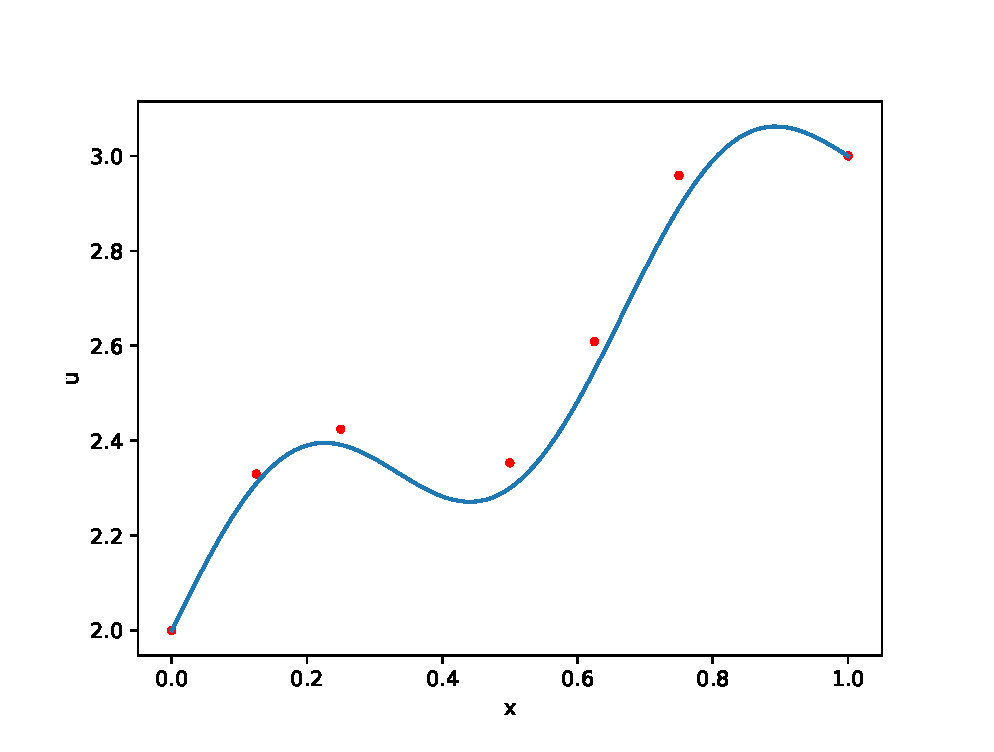
\includegraphics[width=.4\textwidth]{1D_n5} & 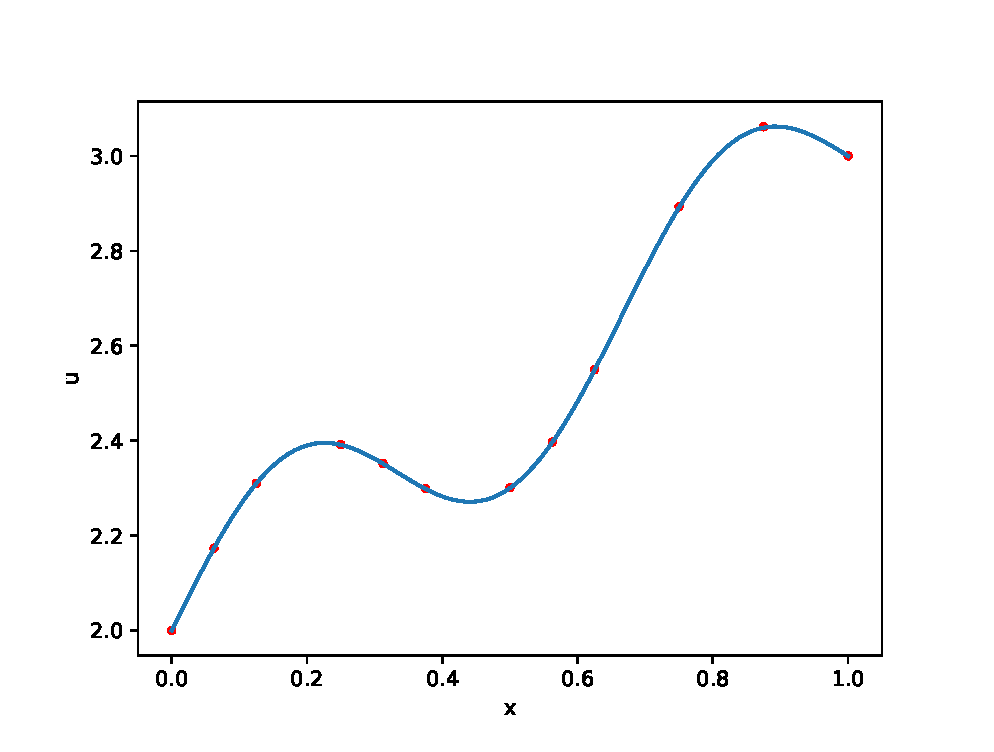
\includegraphics[width=.4\textwidth]{1D_n10} \\
		n=5 & n=10 \\
		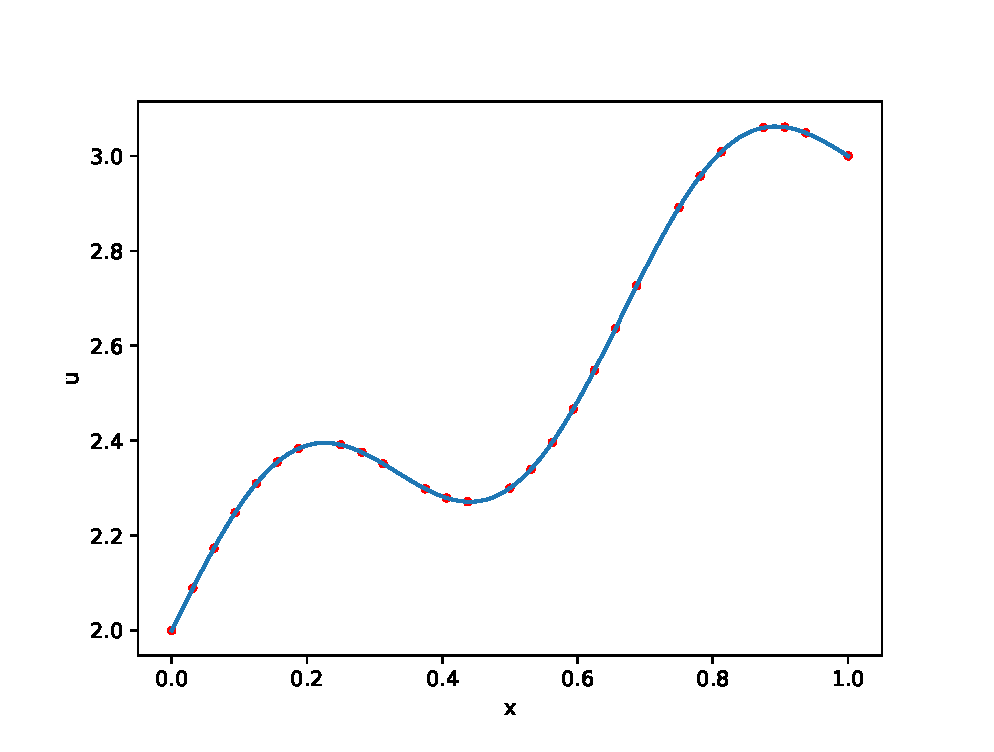
\includegraphics[width=.4\textwidth]{1D_n25} & 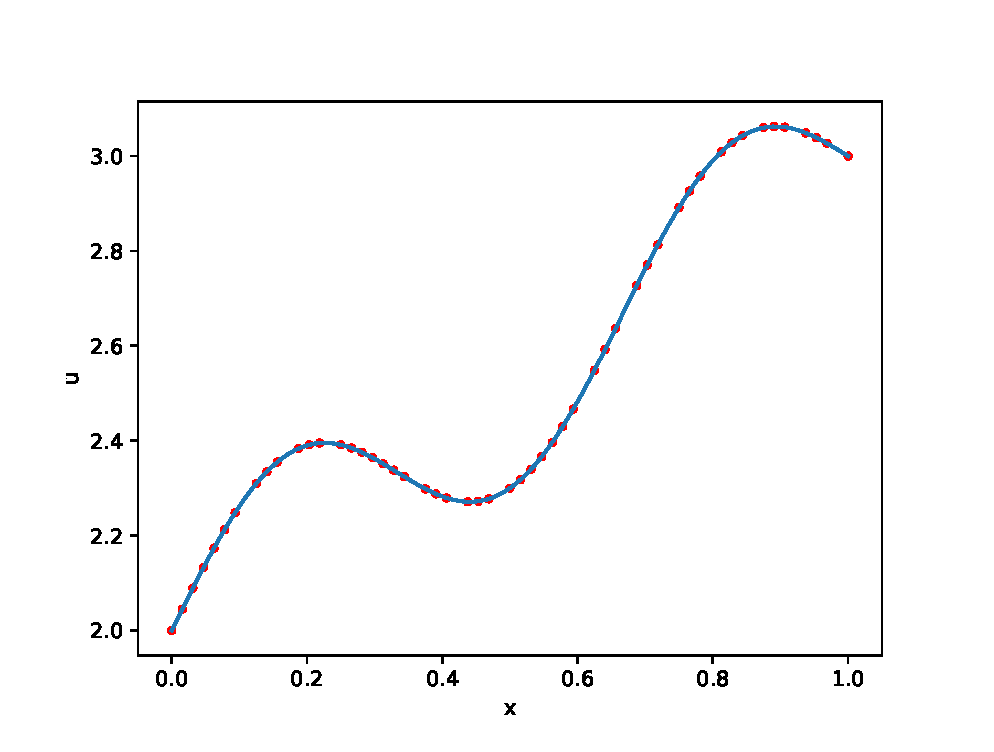
\includegraphics[width=.4\textwidth]{1D_n50} \\
		n=25 & n=50
	\end{tabular}
	\label{1Dsolutions}
	\centering
\end{figure}

A significant advantage of RBF-FD methods is that the formulation does not depend on the domain. Nearly the exact same algorithm can be applied to 2-dimensional problems. \bigbreak

For example, consider the 2-dimensional boundary value problem (Poisson's equation) on the unit disk
\begin{align}
\frac{\partial ^2u}{\partial x^2} + \frac{\partial ^2u}{\partial y^2} &= 0, & u(x,y)&=(y-0.1)^2 \text{ on the boundary}  \label{PDE2D}
\end{align}
The RBF-FD solution can be seen in figure \ref{2Dsolutions} for $n$ points in the interior and sampled at $b$ points on the boundary.

At a given point, it is reasonable to assume that the weights used to approximate the derivative for far off points should be small - essentially that local function values are weighted heavier in the approximation of the derivative. This motivates the idea to use only local points for the calculations of the weights in equation (\ref{row_coef}). In this case we used the $l$-nearest neighbors for each point meaning that each row of $D$ has only $l$ non-zero entries. For large numbers of points, this can dramatically reduce the computational cost of calculating the weights, and also ensures that $D$ is sparse. 

Our implementation uses a variation where we use polyharmonic spline (PHS) RBF kernels augmented with polynomial basis terms, giving a stencil system of the form
$$
\begin{bmatrix}
	A &P\\
	P^T &0
\end{bmatrix}
\begin{bmatrix}
	\vec{\omega}\\
	\vec{\lambda}
\end{bmatrix}
=
\begin{bmatrix}
	L\vec{\phi}(\vec{y}) \\
	L\vec{p}(\vec{y}) 
\end{bmatrix}.
$$
Here $A$ and $L\vec{\phi}(\vec{y})$ are given in (\ref{Amat}) and
\begin{align*}
	P&=
	\begin{bmatrix}
		p_1(\vec{x}_1)  &p_2(\vec{x}_1)  &\cdots  &p_k(\vec{x}_1) \\
		p_1(\vec{x}_2)  &p_2(\vec{x}_2)  &\cdots &p_k(\vec{x}_2) \\
		\vdots  &\vdots  &\ddots &\vdots\\
		p_1(\vec{x}_n)  &p_2(\vec{x}_n)  &\cdots &p_k(\vec{x}_n)
	\end{bmatrix},\\
	L\vec{p}(\vec{y}) ^T&=\begin{bmatrix}
		L p_1(\vec{x})\vert_{\vec{x}=\vec{y}}  &L p_2(\vec{x})\vert_{\vec{x}=\vec{y}} &\cdots &L p_k(\vec{x})\vert_{\vec{x}=\vec{y}} 
	\end{bmatrix}
\end{align*}
where $\{p_i(\vec{x})\}_{i=1}^d$ are polynomial basis terms.

The vectors of weights, $\mathbf{\omega}\omega$, then become the rows of our differentiation matrix, $D$. Once $D$ is formed, we have reduced the problem to that of solving the linear system $D\vec{u} = \vec{f}$. \bigbreak

\begin{figure}[h]
	\begin{tabular}{cc}
		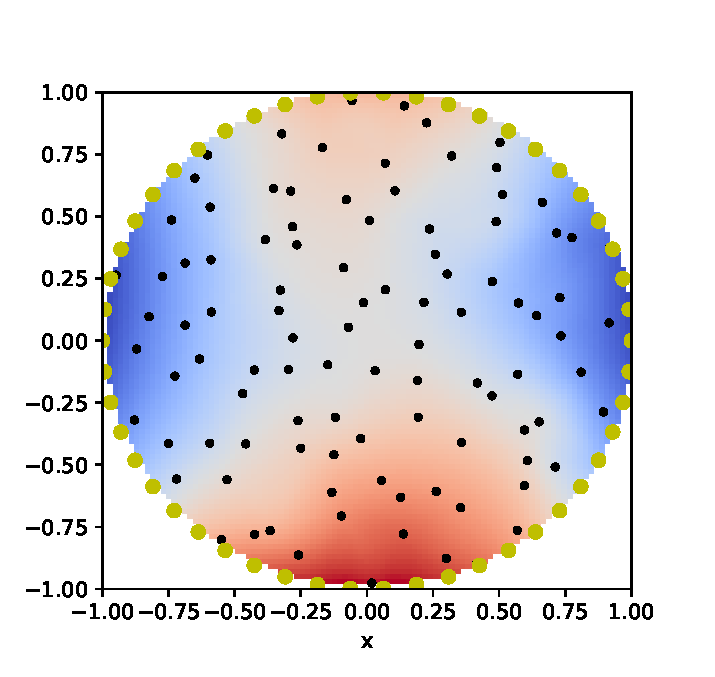
\includegraphics[width=.5\textwidth]{2D_n100_b50} & 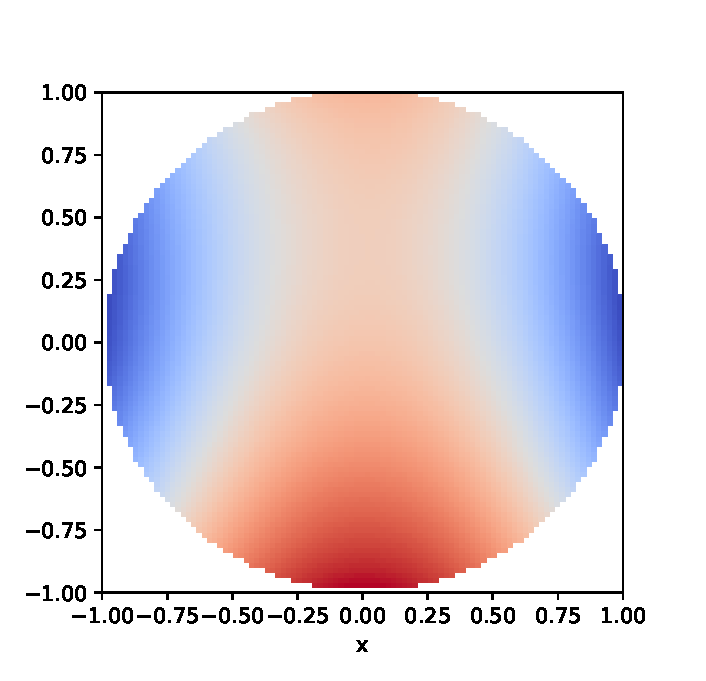
\includegraphics[width=.5\textwidth]{2D_n2000_b50_l50} \\
		n=100 \phantom{==} b=50 \phantom{==} l=5 & n=2000 \phantom{==} b=50 \phantom{==} l=50 
	\end{tabular}
	\caption{Solution to (\ref{PDE2D}) using $n$ interior points (black), $b$ boundary points (gold), and a stencil size of $l$ nearest neighbors}
	\label{2Dsolutions}
	\centering
\end{figure}

%%%%%%%%%%%%%%%%%%%%%%%%%%%%%%%%%%%%%%%%%%%%%%%%%%%%%%%%%%%%%%%
%%%%%%%%%%%%%%%%%%%%%%%%%%%%%%%%%%%%%%%%%%%%%%%%%%%%%%%%%%%%%%%
%%%%%%%%%%%%%%%%%%%%%%%%%%%%%%%%%%%%%%%%%%%%%%%%%%%%%%%%%%%%%%%
\section{Methods}

	The method can be separated into three steps: generating points, forming the differentiation matrix, and either solving the resulting sparse system or use it to step through time-dependent problems. While Bollig, Flyer, and Erlebacher\cite{Bollig2012} implement time stepping in parallel over multiple CPUs and GPUs, they did not parallelize the calculation of the differentiation matrix. In addition to this, Flyer et al. \cite{Flyer2016-1}\cite{Flyer2017-2} and Barnett \& Wicker \cite{FlyerBarnettWicker2016} explored using a particular kind of RBF called polyharmonic spline (PHS) radial basis functions in RBF-FD, but they did not implement their techniques in parallel.
	
	For this project, we wanted to parallelize the generation of the differentiation matrix in the RBF-FD method using polyharmonic spline RBF kernels augmented with polynomial basis terms. The choice of points has a large effect on these later two steps however, so a discussion on their generation is in order.

%%%%%%%%%%%%%%%%%%%%%%%%%%%%%%%%%%%%%%%%%%%%%%%%%%%%%%%%%%%%%%%
\subsection{Generating and Ordering Points}
The first step is to choose a set of points on which to approximate the solution. Classical finite difference methods require points to be from a uniform grid over the domain. This is limiting in that it requires the number of points to be an integer power of the dimension of the domain (before applying a mask to remove points outside of the domain) and that it requires the points to be at particular locations. For RBF-FD we are completely unrestricted. The freedom to choose the number of points is purely beneficial, and it is particularly nice that it does not rely on the dimensions of the space, however the freedom to choose points arbitrarily begs the question: what are the best points to choose?

The theory suggests that the points should sample the entire domain. The choice to use polynomial basis terms adds restrictions to the choice of points. If all the points in a particular stencil lie along a line for example, the $1, x$, and $y$ columns will be linearly dependent. This would suggest the use of a random set of points, to make such linear dependencies unlikely. 

It is desirable to have the distances between points in the stencil somewhat regular however. Consider fixing all points except one. Then as the free point approaches one of the points in its stencil, the corresponding column in the stencil matrix will approach the first column in the matrix (corresponding to the free point at the stencil center) thus making the matrix increasingly ill-conditioned. In other words, we would like the distances between points to vary but not by significant orders of magnitude. The pseudorandom Halton points\cite{Halton1960} do this job nicely. These points are generated by a process involving primes to distributed them across the unit square. We then map them to the disk by the area-preserving transformation $f(x, y) = \langle \sqrt{x}\cos(2\pi y), \sqrt{x}\sin(2 \pi y) \rangle$.


In figure \ref{randomhalton} can be seen one hundred points chosen randomly on the left and one hundred Halton points (generated by \cite{Burkardt2016}) on the right. The Halton points appear random but also avoid clustering.

\begin{figure}[h]
	\centering
	\begin{tabular}{cc}
		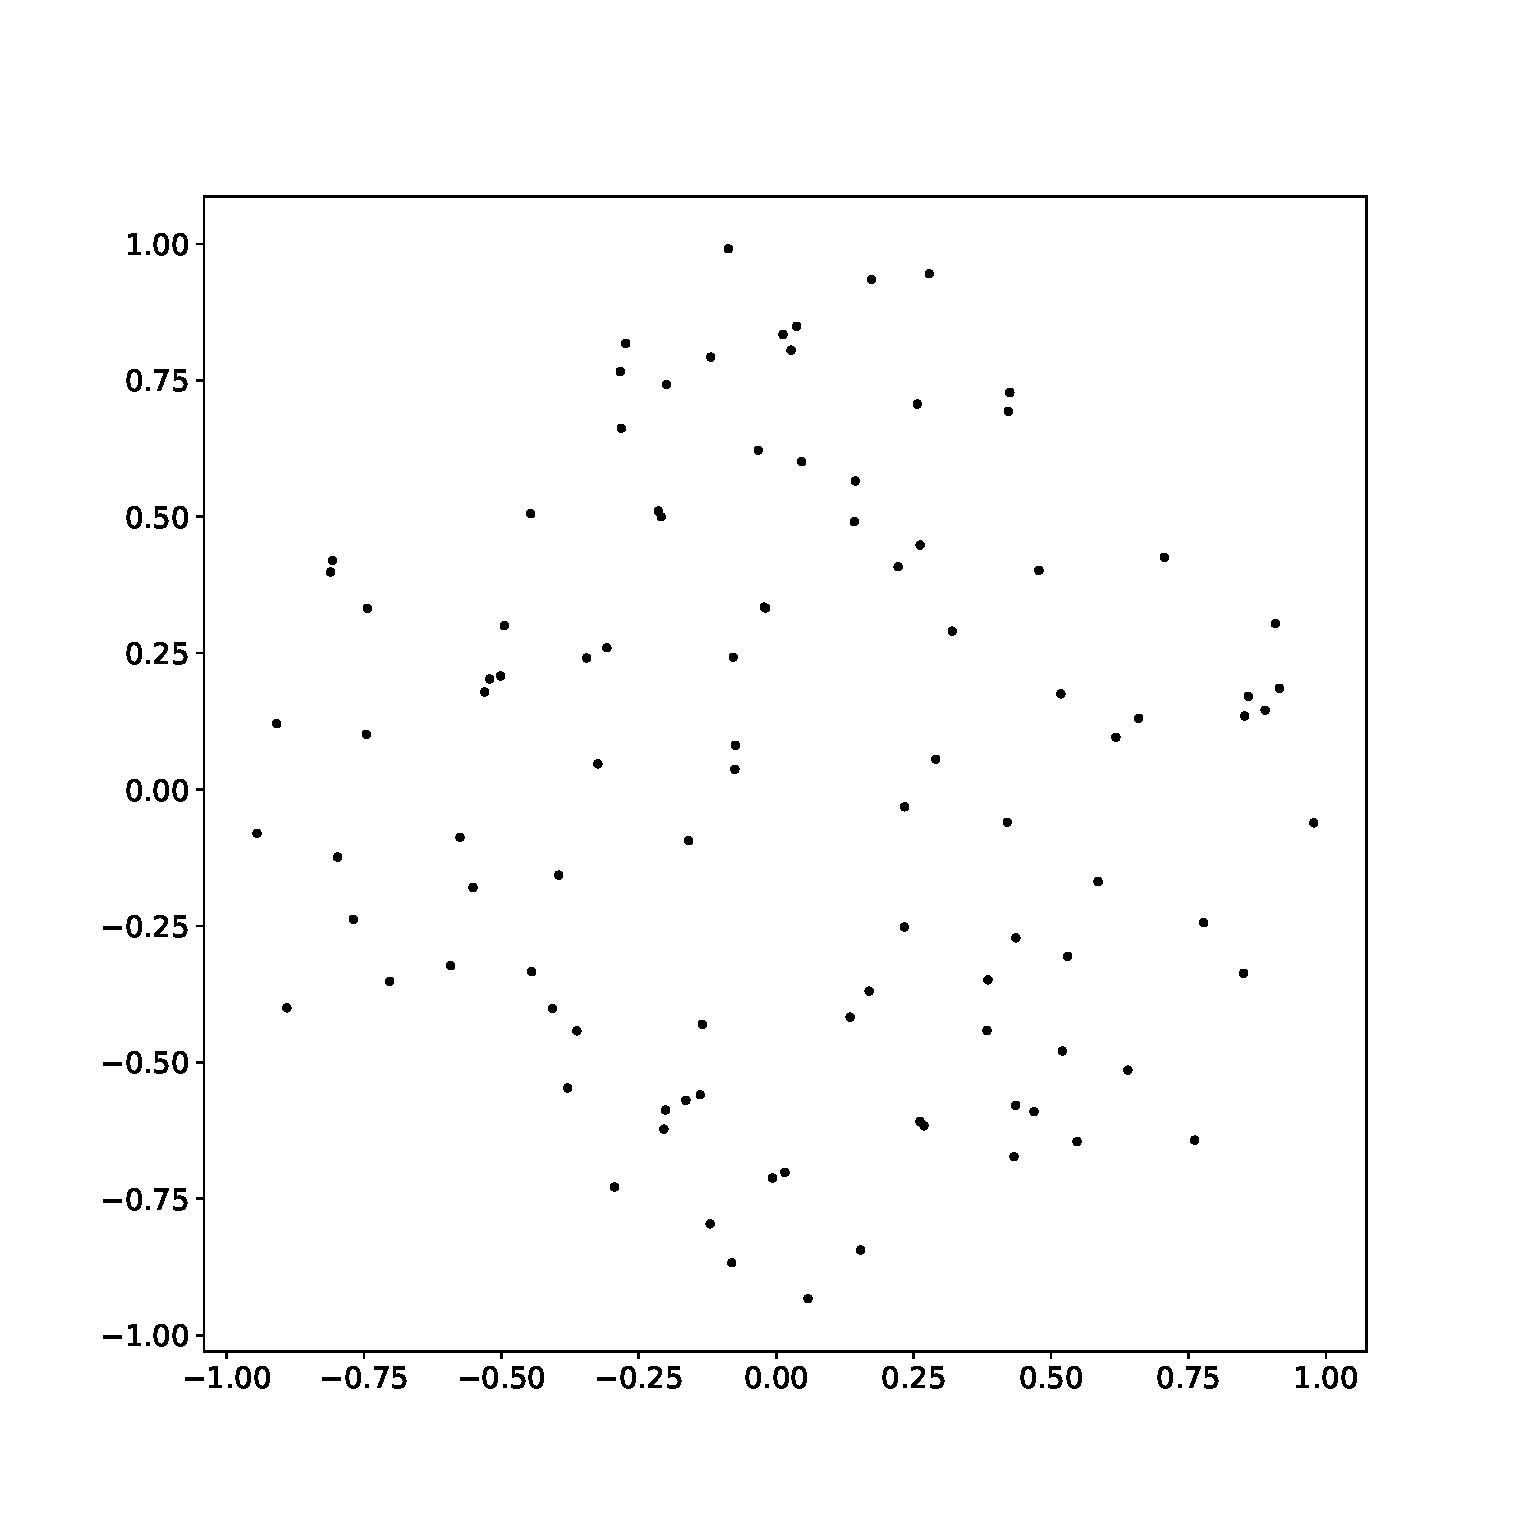
\includegraphics[width=.5\textwidth]{random_100_disk.eps} & 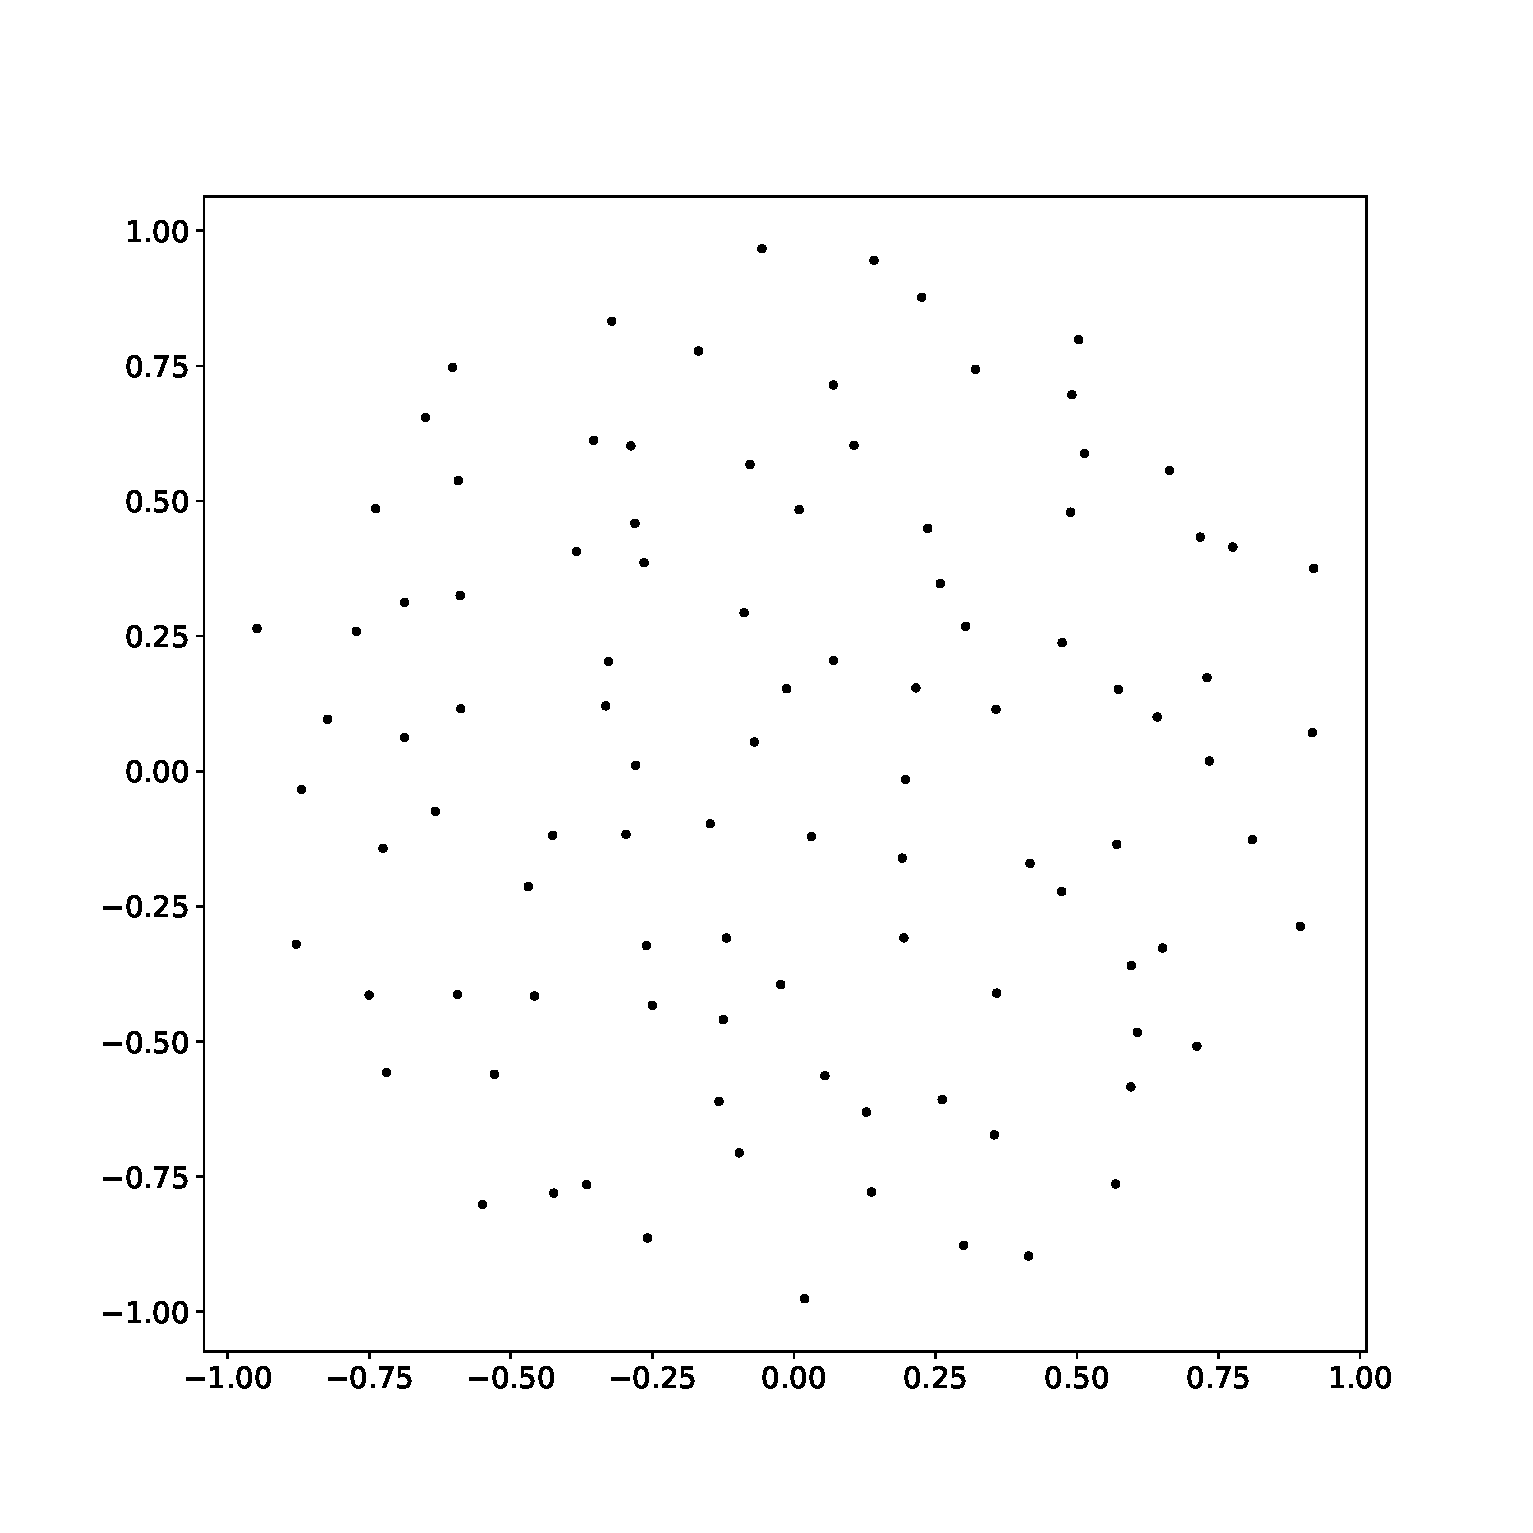
\includegraphics[width=.5\textwidth]{halton_100_disk.eps} \\
	\end{tabular}
	\caption{Random points (left) and pseudorandom Halton points (right) on the unit disk.}
	\label{randomhalton}
\end{figure}

Another option we explored was using the Vogel nodes as seen in figure \ref{vogel}. These points seem to be more regularly spaced. They are generated by choosing points on a spiral defined as

$$
\vec{x}_i = \left( \sqrt{\frac{i}{n}}\cos(i\hat{\theta}), \sqrt{\frac{i}{n}}\sin(i\hat{\theta})  \right) \phantom{==}\text{for } i = 1, 2, \dots, n
$$
where the constant $\hat{\theta} = \pi (3-\sqrt{5})$. Their spiral nature becomes more obvious as the number of points is increased. The figure \ref{vogel} shows one hundred Vogel nodes on the unit disk, the spiral used to generate them, and one thousand Vogel nodes on the unit disk.

\begin{figure}
	\centering
	\begin{tabular}{ccc}
		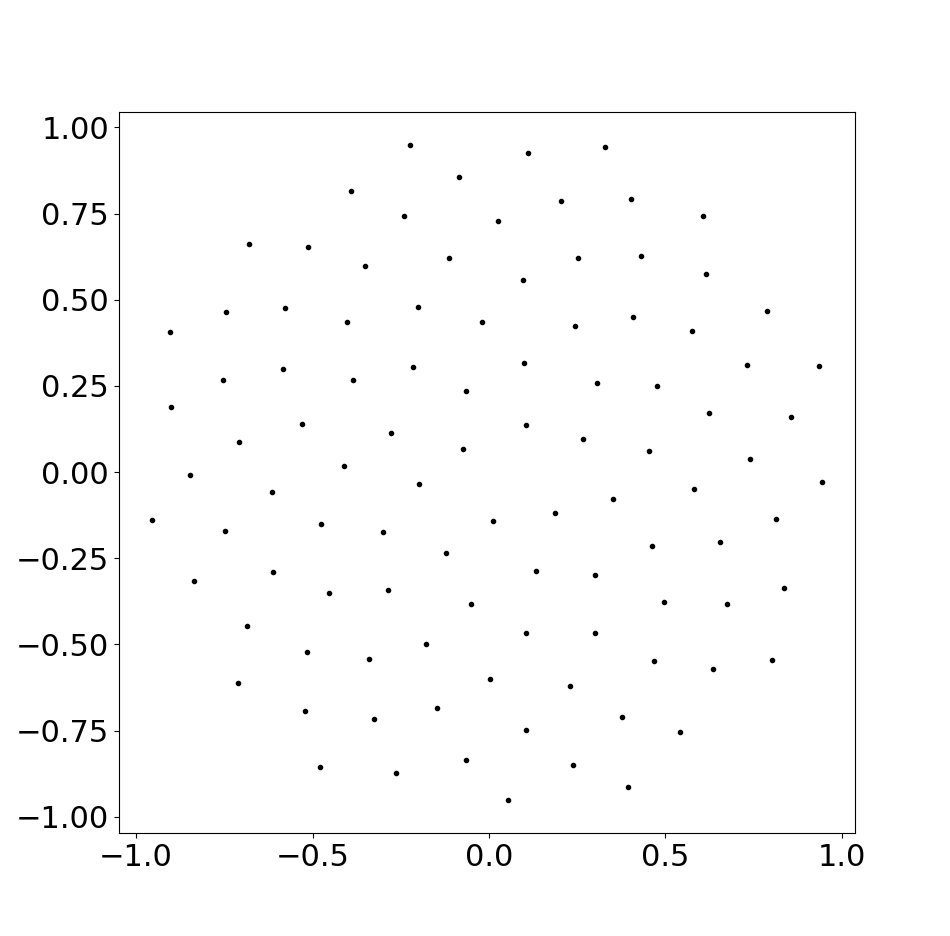
\includegraphics[width=.3\textwidth]{vogel_no_spiral.png} & 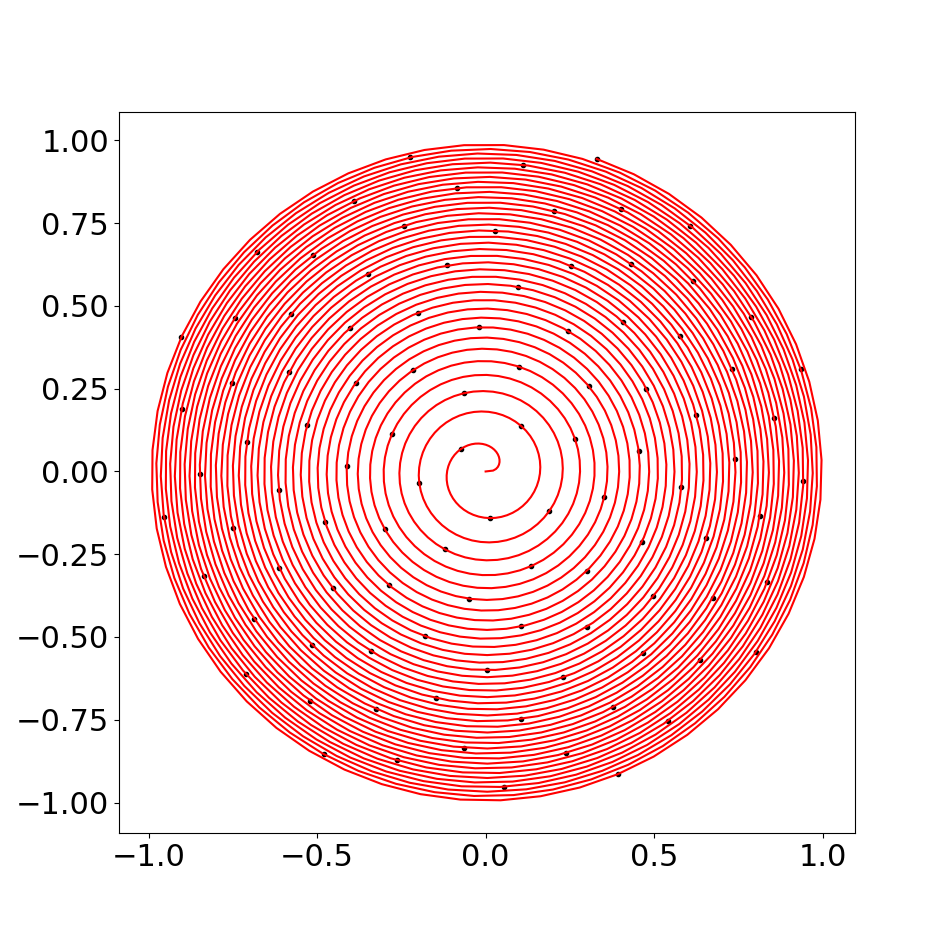
\includegraphics[width=.3\textwidth]{vogel_spiral.png} &
		%\multicolumn{2}{c}{
		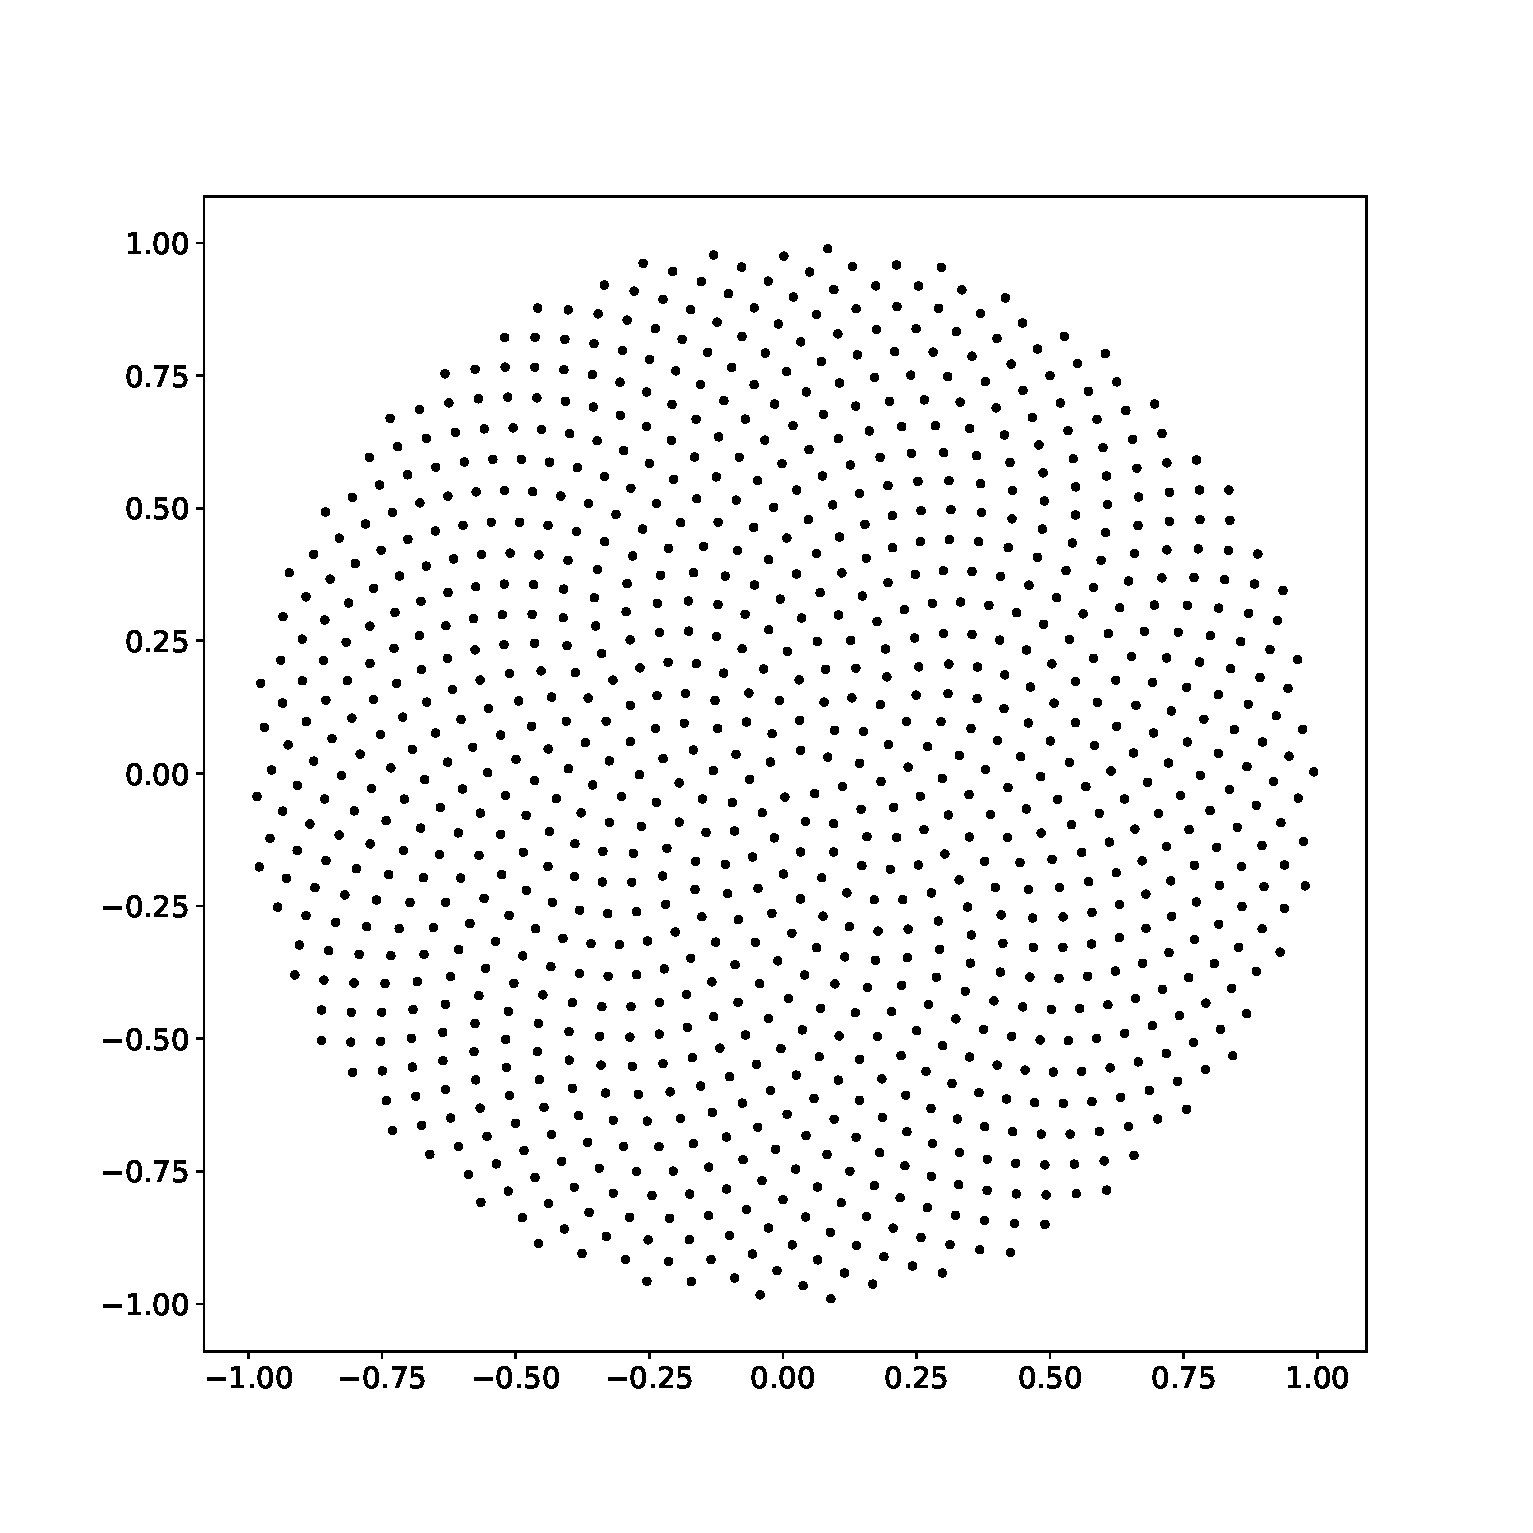
\includegraphics[width=.3\textwidth]{vogel_1000_disk.eps} 
		%}\\
	\end{tabular}
	\caption{One hundred Vogel nodes on the unit disk (left), the spiral used to generate them (center), and one thousand Vogel nodes on the unit disk (right).}
	\label{vogel}
\end{figure}

Once the points are chosen we use a KD-tree to calculate nearest neighbors then the weights are generated and used to form a sparse matrix. In general the sparsity will not follow a particular pattern. The first point in the list may be near to the fifth, twentieth, or two hundredth points. The first column in figure \ref{orderings} shows the sparsity pattern for our three point distributions.

These sparsity patterns become important when we parallelize matrix-vector multiplication. If a matrix system is to be divided up among four processes it is natural to chunk the matrix and vectors up along contiguous rows as seen in the sparsity pattern and in the coloring of the block matrix below.

$$
\begin{bmatrix}
	{\color{red} A_{11} } & {\color{red} A_{12} } & {\color{red} A_{13} } & {\color{red} A_{14} }\\
	{\color{green} A_{21} } & {\color{green} A_{22} } & {\color{green} A_{23} } & {\color{green} A_{24} } \\
	{\color{blue} A_{31} } & {\color{blue} A_{32} } & {\color{blue} A_{33} } & {\color{blue} A_{34} } \\
	{\color{black} A_{41} } & {\color{black} A_{42} } & {\color{black} A_{43} } & {\color{black} A_{44} } \\
\end{bmatrix}
\begin{bmatrix}
	{\color{red} \vec{x}_{1} } \\
	{\color{green} \vec{x}_{2} } \\
	{\color{blue} \vec{x}_{3} } \\
	{\color{black} \vec{x}_{3} } 
\end{bmatrix}
=
\begin{bmatrix}
	{\color{red} \vec{b}_{1} } \\
	{\color{green} \vec{b}_{2} } \\
	{\color{blue} \vec{b}_{3} } \\
	{\color{black} \vec{b}_{3} }
	\end{bmatrix}
$$
\begin{center}
	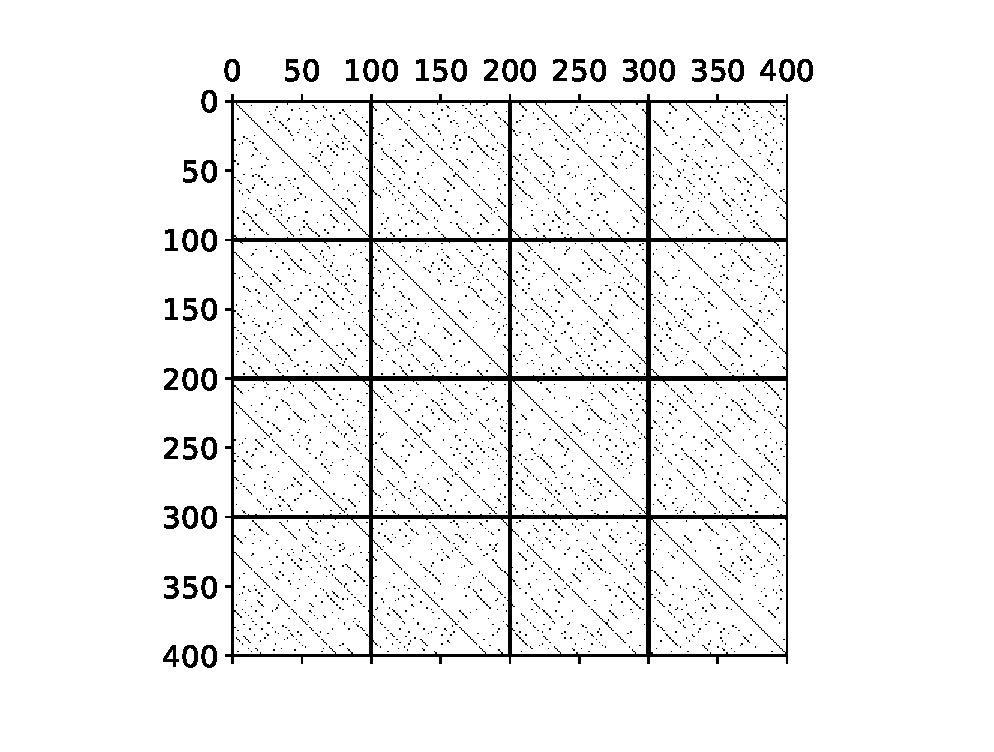
\includegraphics[width=.5\textwidth]{spy_halton_chunked.eps}
\end{center}


%\begin{wrapfigure}[5]{r}{0.5\textwidth}
%\begin{center}
%        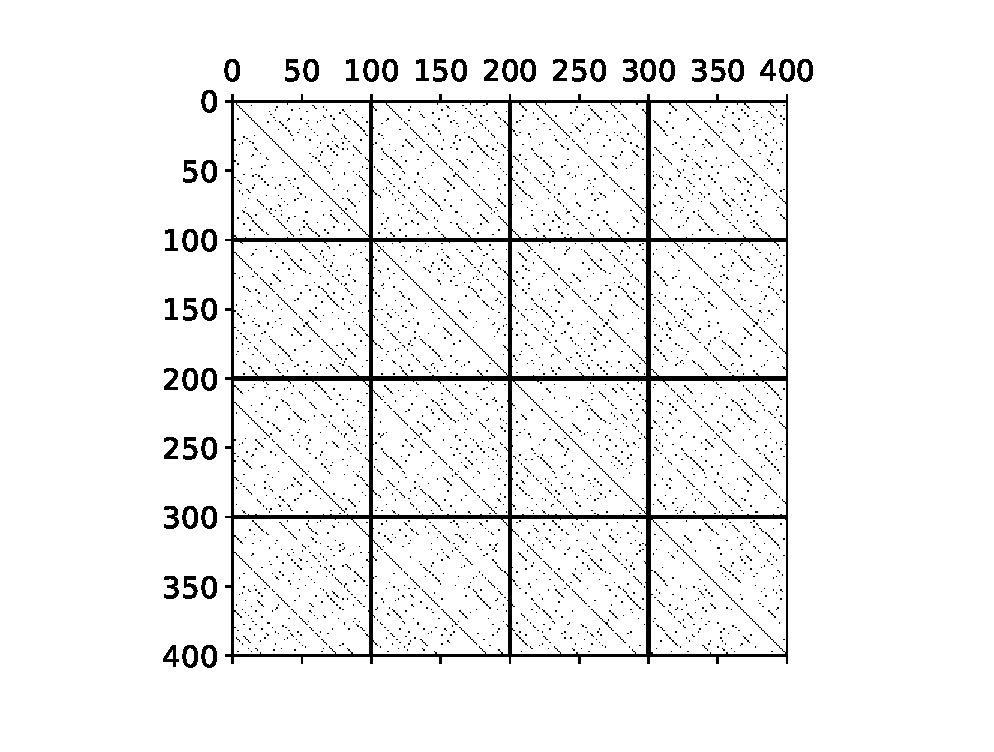
\includegraphics[width=0.5\textwidth]{spy_halton_chunked.eps}
%\end{center}
%    \caption{A gull}
%\end{wrapfigure}
%\begin{figure}[Hb]
%	\centering
%\begin{tabular}{cc}

%&
%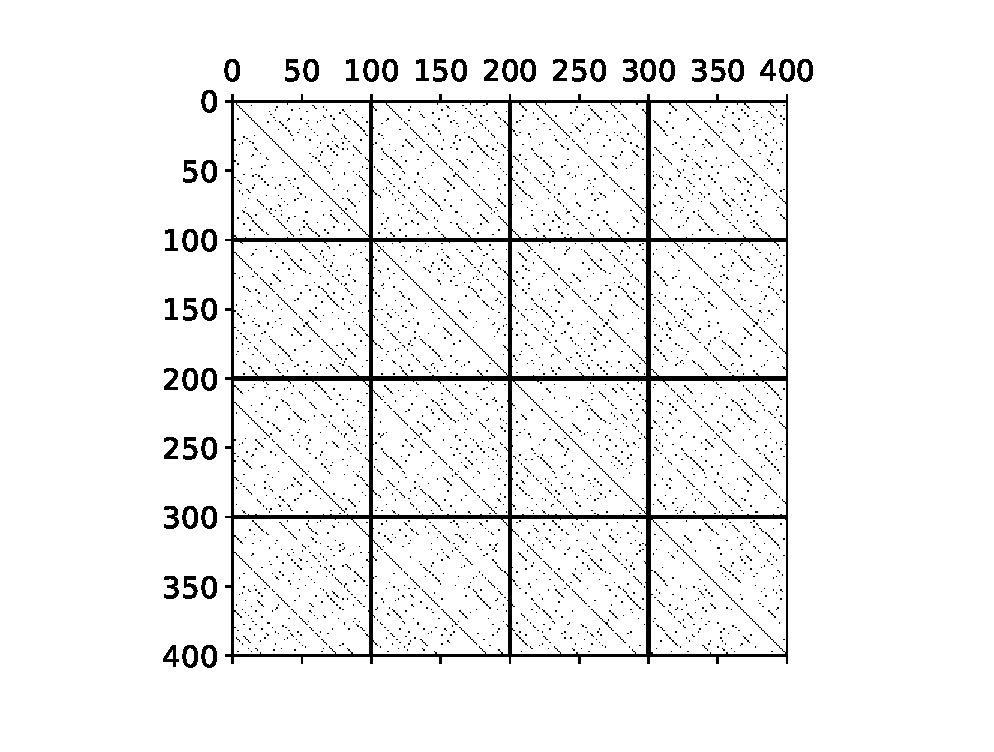
\includegraphics[width=.4\textwidth]{spy_halton_chunked.eps}
%\end{tabular}
%\caption{One hundred Vogel nodes on the unit disk (top left), the spiral used to generate them (top right), and one thousand Vogel nodes on the unit disk (bottom).}
%\label{halton_chunked}
%\end{figure}



If the red process has the matrices $A_{11}, A_{12}, A_{13}, A_{14}$, and the vector $\vec{x}_1$ stored in memory, then in order to calculate $\vec{b}_1$ it will need need to communicate with the green, blue, and black processes to get the vectors $\vec{x}_2, \vec{x}_3$, and $\vec{x}_4$ respectively. This communication is expensive and can be reduced by taking advantage of the geometry of the problem.

Consider dividing the domain among two processes vertically so that process one is responsible for nodes in the right half-plane and process two is responsible for nodes in the left half plane. Figure \ref{dsik_two_proc} illustrates this, where process one is responsible for the red nodes and process two is responsible for the blue nodes and the green nodes. Some of the points in the left half plane will be nearest neighbors of points in the right half plane (depicted in green). It would be advantageous if each process had it's nodes organized so all of the values that needed to be shared with neighboring processes were contiguous in memory. These green nodes would correspond to non-zero entries outside of the diagonal blocks of the matrix.

\begin{figure}[!b]
	\centering
	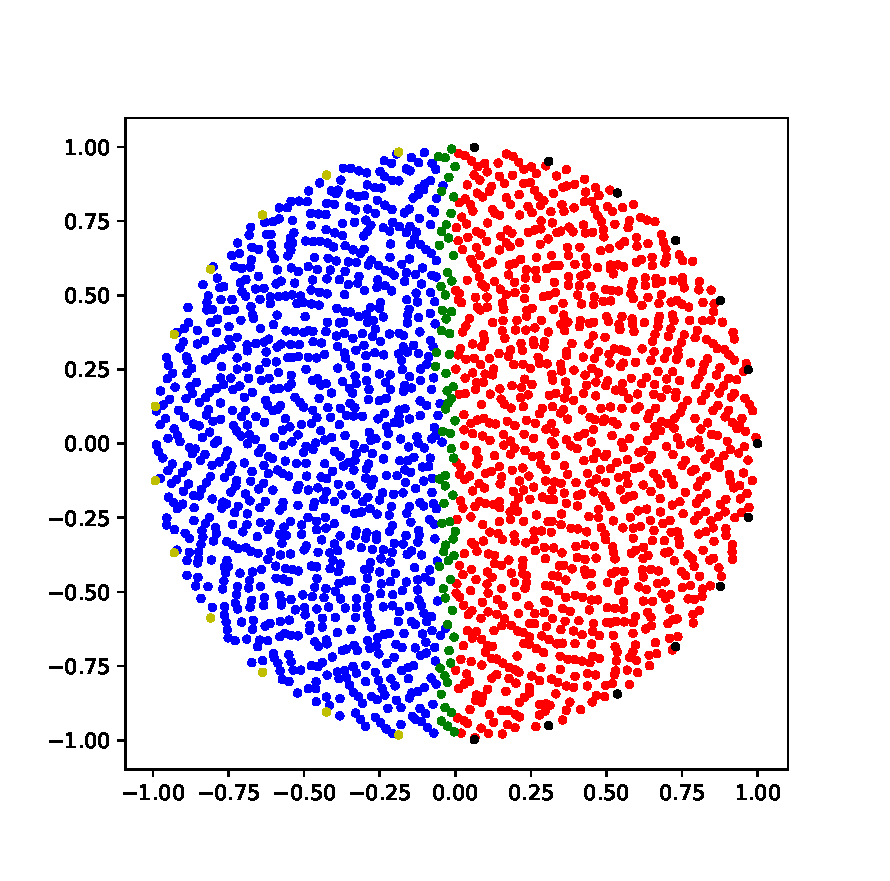
\includegraphics[width=.5\textwidth]{nearest_2proc_disk.eps}
	\caption{Partitioning of the domain }
	\label{dsik_two_proc}
\end{figure}

Figure \ref{decomp_strategies} shows four ways to divide the disk into equal area domains. When the points are ordered according to color the off diagonal blocks of the differentiation matrix are very sparse or even empty. For example, the stripes pattern at the top left of figure \ref{decomp_strategies} would result in the red-black and black-red blocks of the matrix being completely empty since no red point is a nearest neighbor of a black point and vice versa. 

\begin{figure}[ht]
	\centering
	\begin{tabular}{cc}
		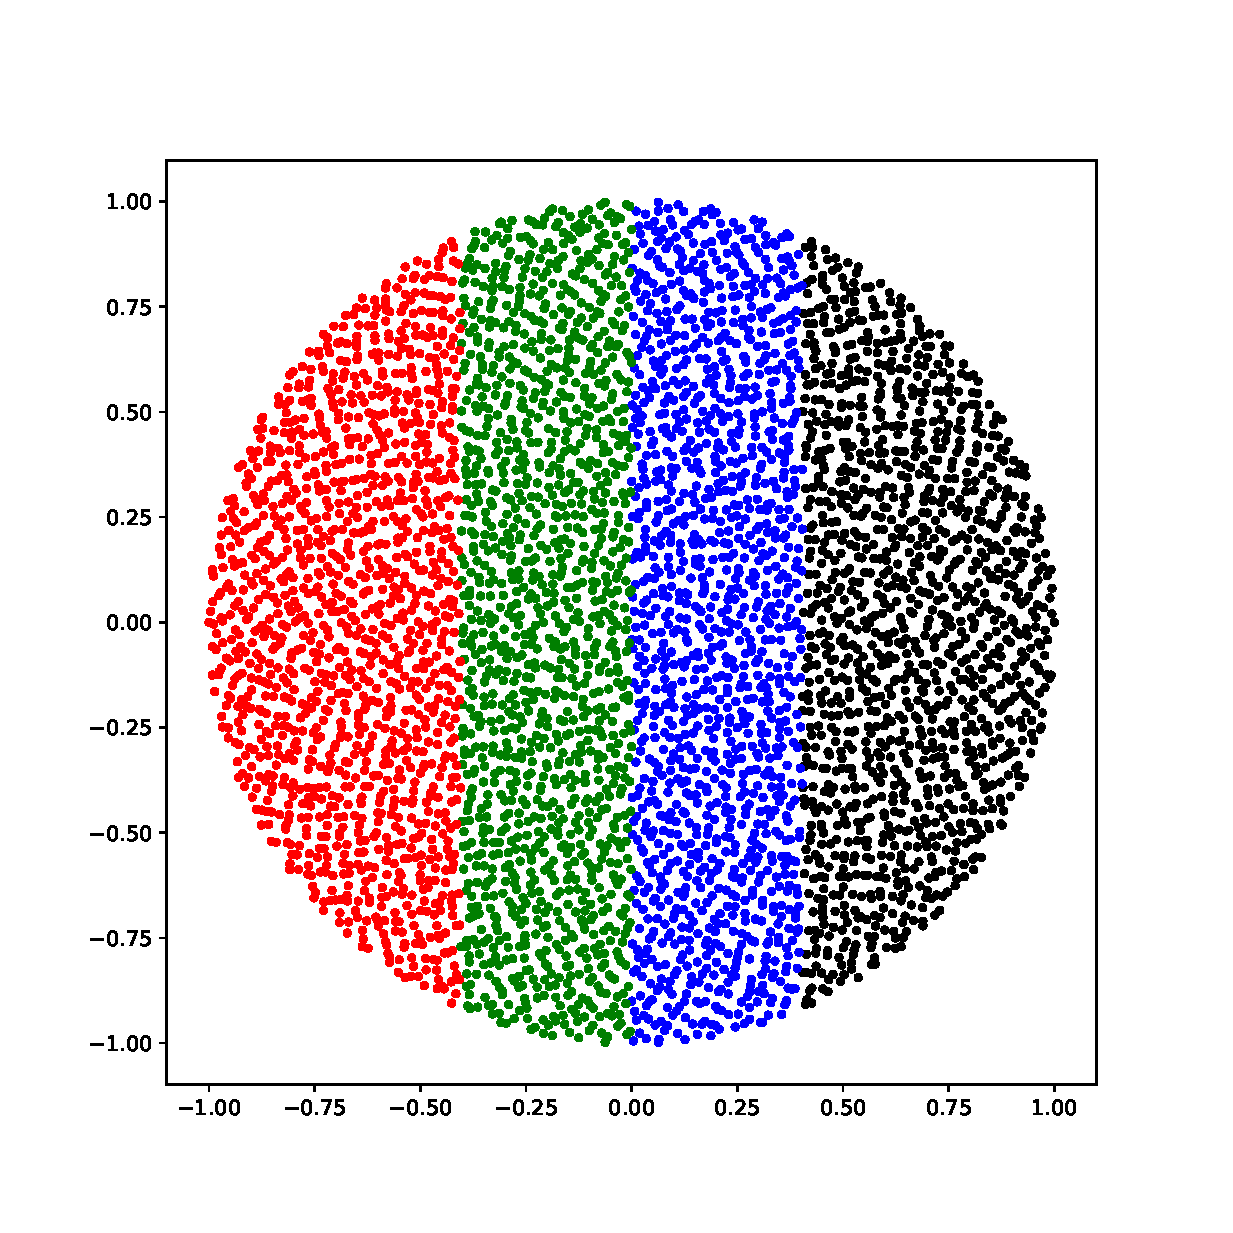
\includegraphics[width=.4\textwidth]{disk_decomp_strips.eps} & 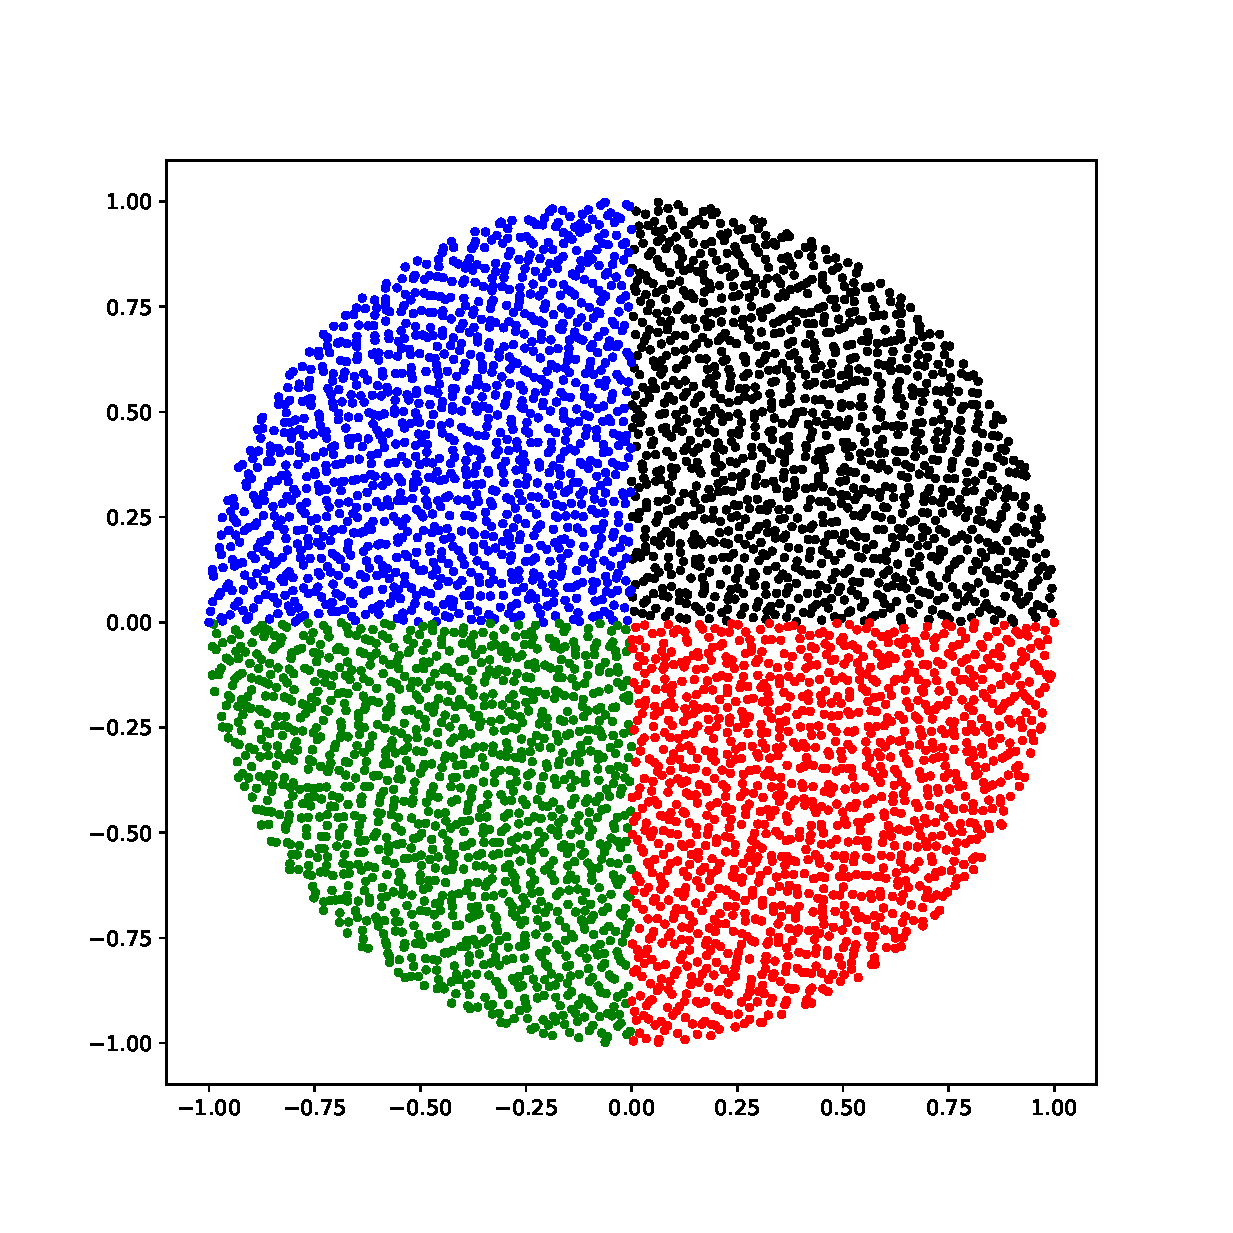
\includegraphics[width=.4\textwidth]{disk_decomp_quad.eps} \\
		Stripes & Quadrants \\
		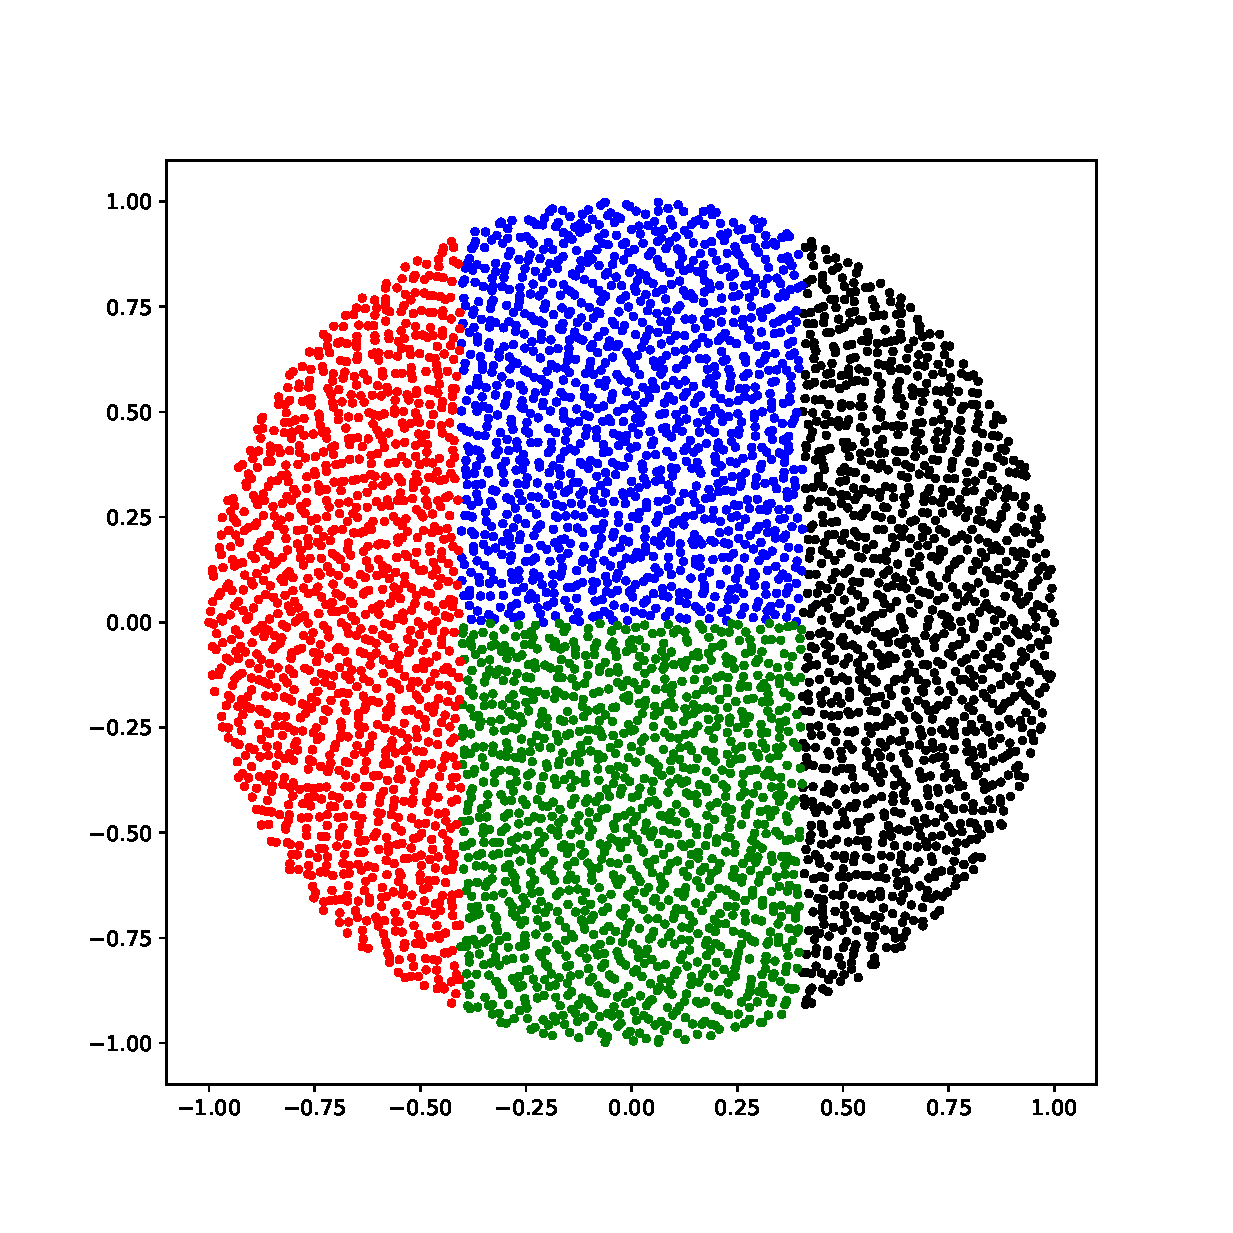
\includegraphics[width=.4\textwidth]{disk_decomp_cake.eps} & 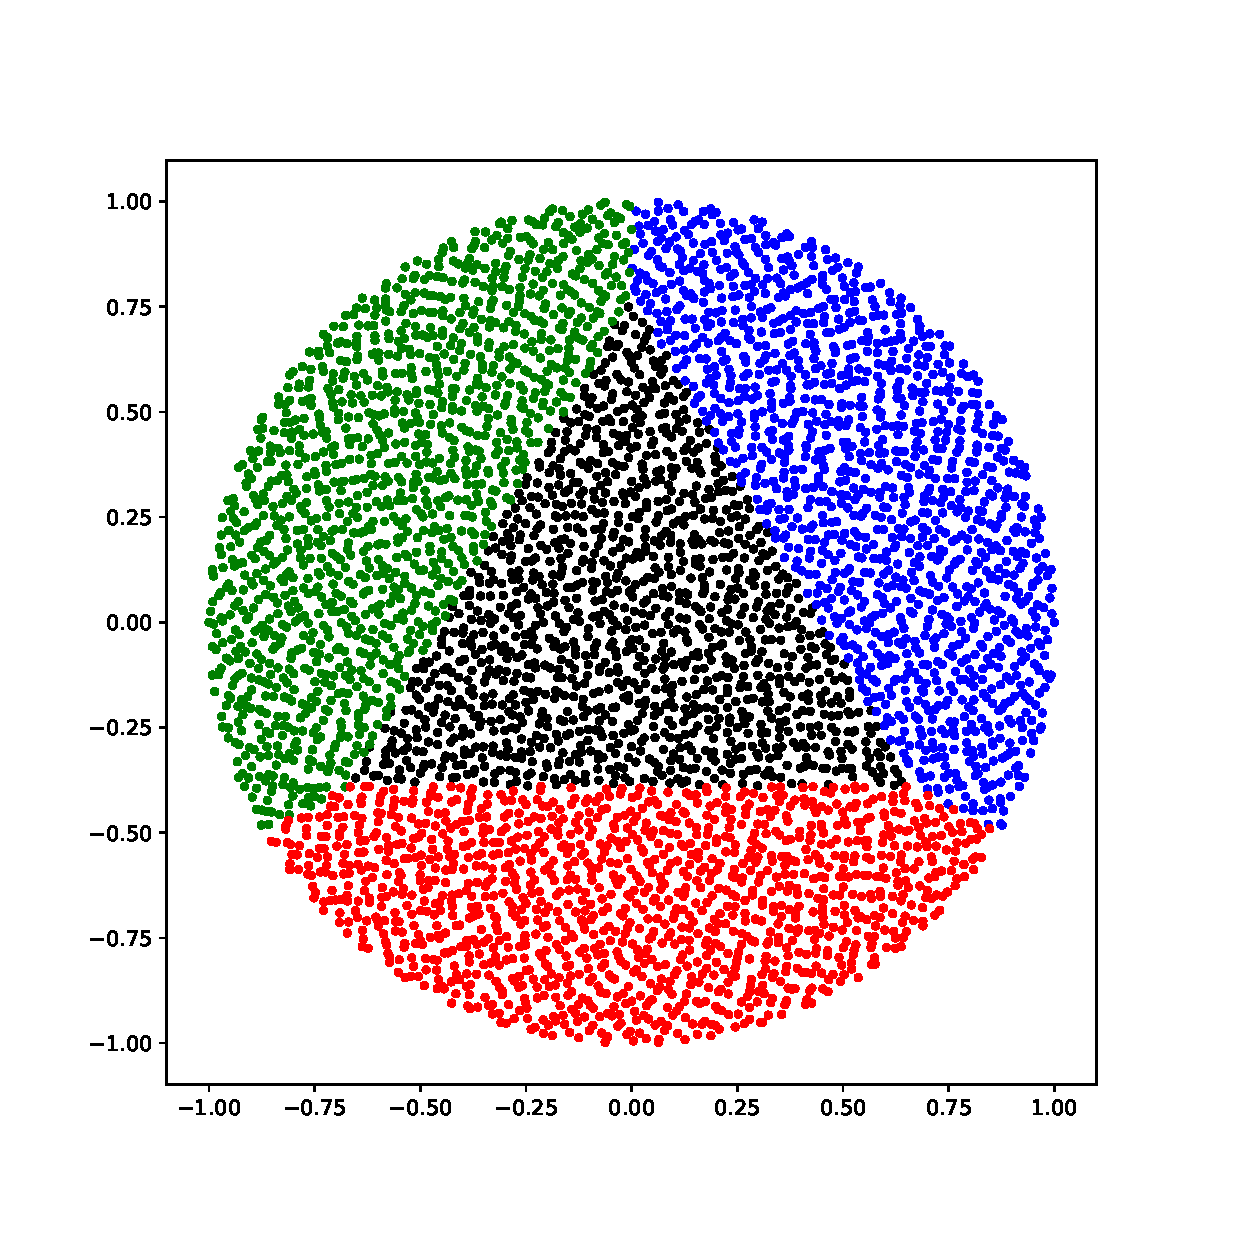
\includegraphics[width=.4\textwidth]{disk_decomp_triangle.eps} \\
		Cake-cutting & Triangle-cutting
	\end{tabular}
	\caption{Four ways to partition the disk with equal area.} \label{decomp_strategies}
\end{figure}

These decomposition strategies lead to a trade off. When the partitions are separated (as the red and black are in the Stripes and Cake-Cutting patterns) they will not need to communicate nearest neighbors (provided the stencil doesn't get too large). The amount of data that needs to be communicated is  proportional to the length of the boundaries between processes. Since initiating communications has a high overhead in MPI and the overhead increases only marginally as the amount of data increases, we have decided to focus on the Stripes pattern. A stronger condition than ordering the points along colors of equal area vertical stripes is to order them in order of increasing $x$ value. This is far simpler to code and can be done in $\mathcal{O}(n\log n)$ time on average. 

Lastly there is an ordering called the Reverse Cuthill-McKee that is a general ordering scheme for sparse matrices. Since we were trying to reduce the bandwidth of the matrix we visually compared the sparsity pattern to that of the $x$-ordering. The results can be seen in figure \ref{orderings}.

\newcommand{\figordersize}{.25}
\begin{figure}[h]
	\centering
	\begin{tabular}{cc}
		Random & \begin{tabular}{ccc}
			Unordered & $x$ Ordering & RCM Ordering \\
			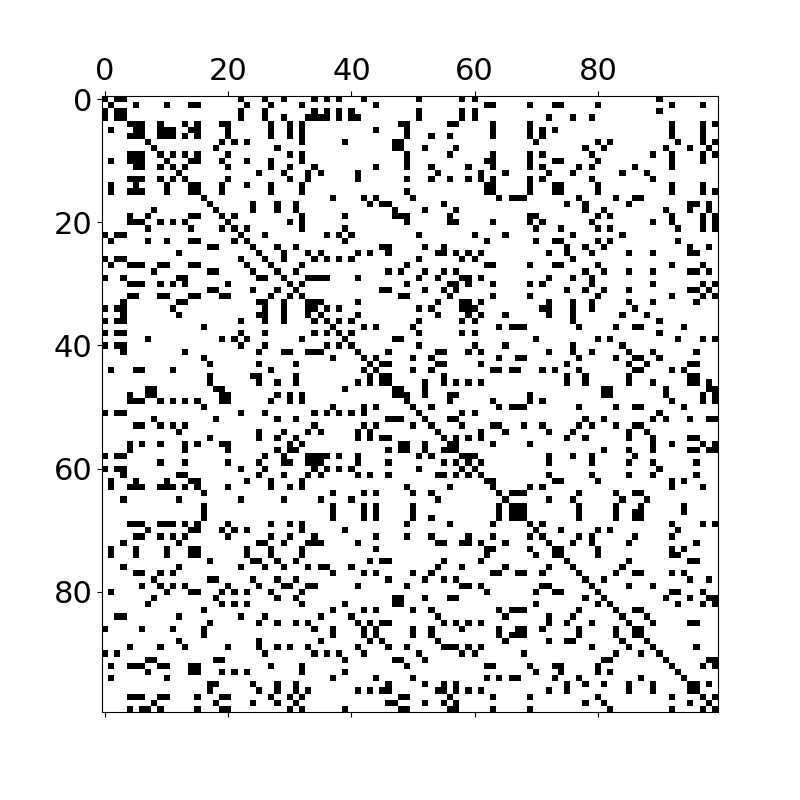
\includegraphics[width=\figordersize\textwidth]{spy_random_unordered.png} &
			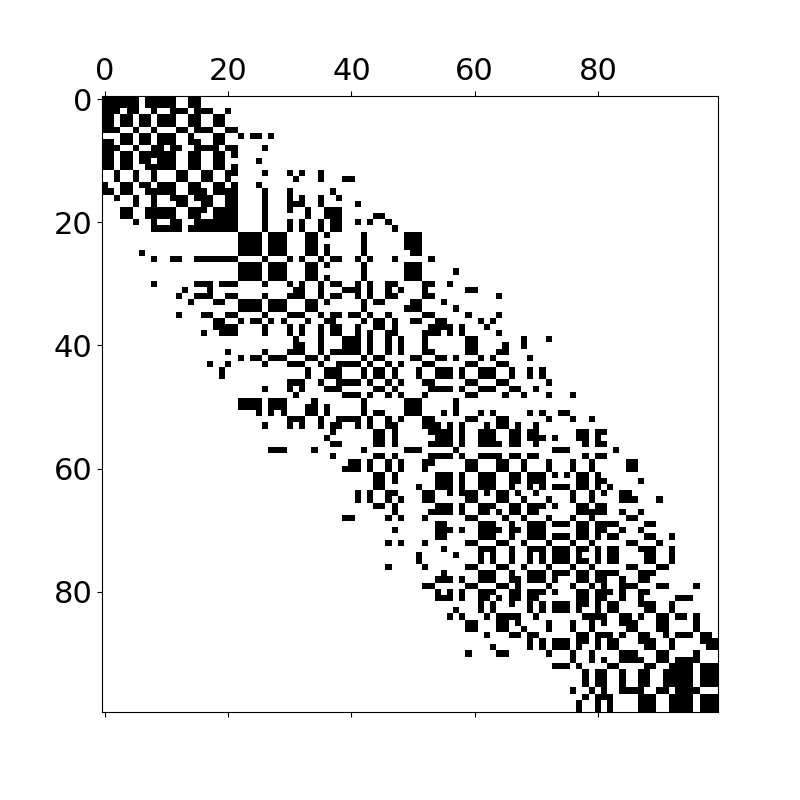
\includegraphics[width=\figordersize\textwidth]{spy_random_xorder.png} &
			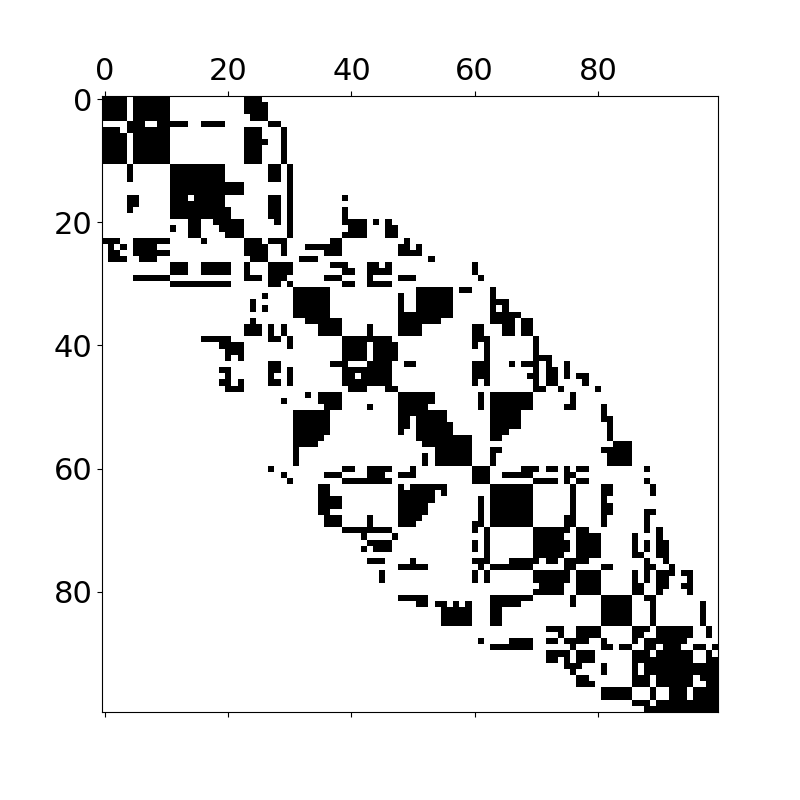
\includegraphics[width=\figordersize\textwidth]{spy_random_rcm.png} \end{tabular} \\
		Halton & \begin{tabular}{ccc}
			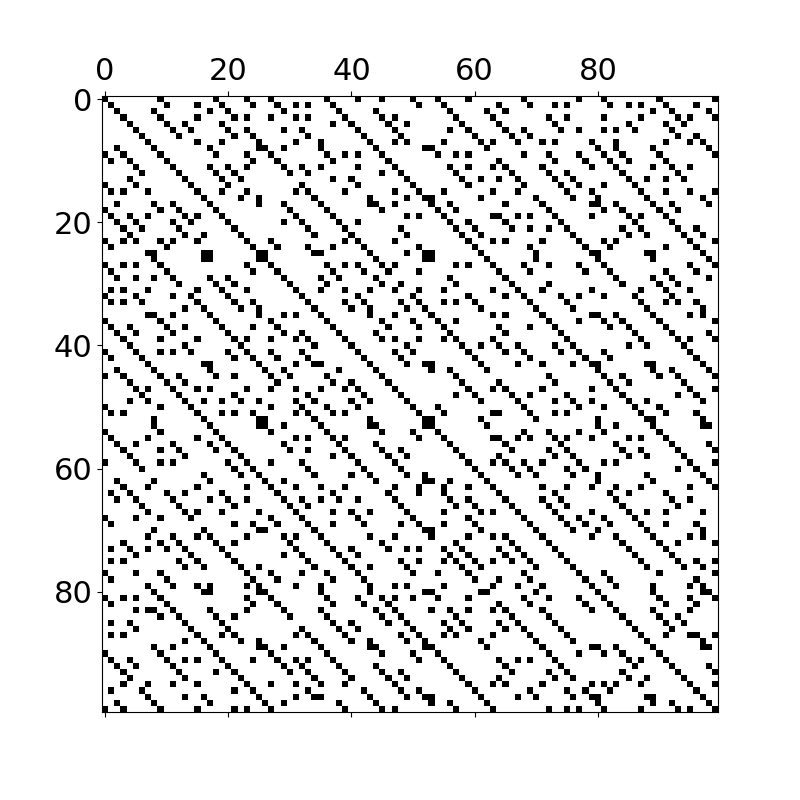
\includegraphics[width=\figordersize\textwidth]{spy_halton_unordered.png} &
			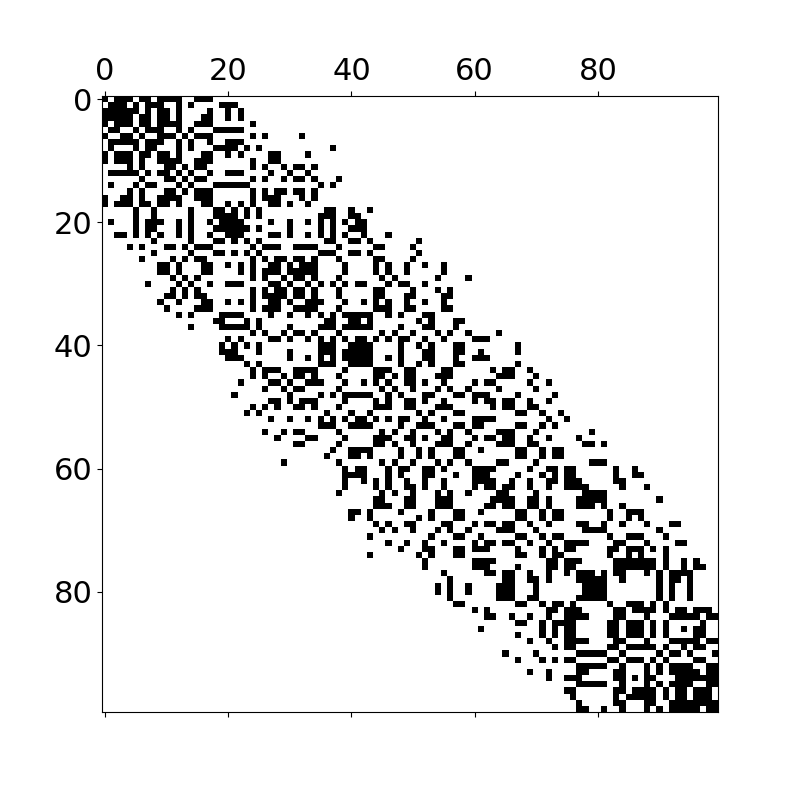
\includegraphics[width=\figordersize\textwidth]{spy_halton_xorder.png} &
			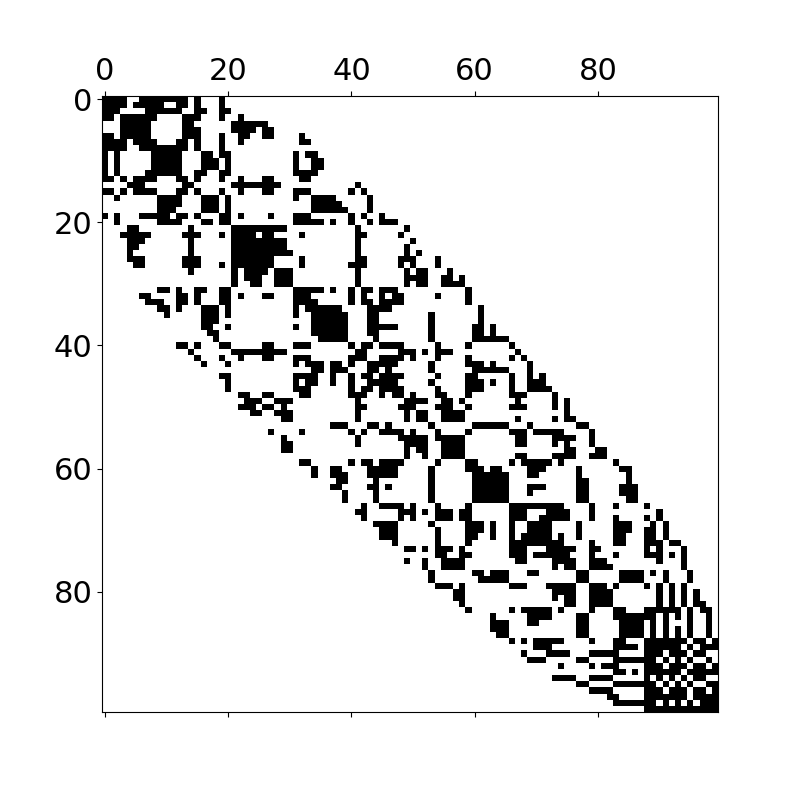
\includegraphics[width=\figordersize\textwidth]{spy_halton_rcm.png} \end{tabular} \\
		Vogel & \begin{tabular}{ccc}
			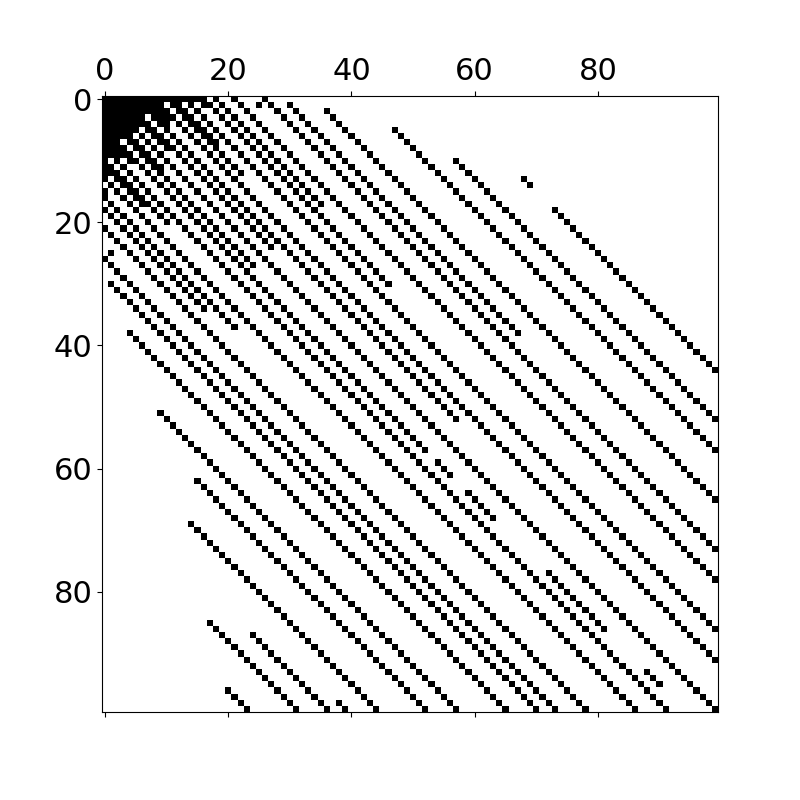
\includegraphics[width=\figordersize\textwidth]{spy_vogel_unordered.png} &
			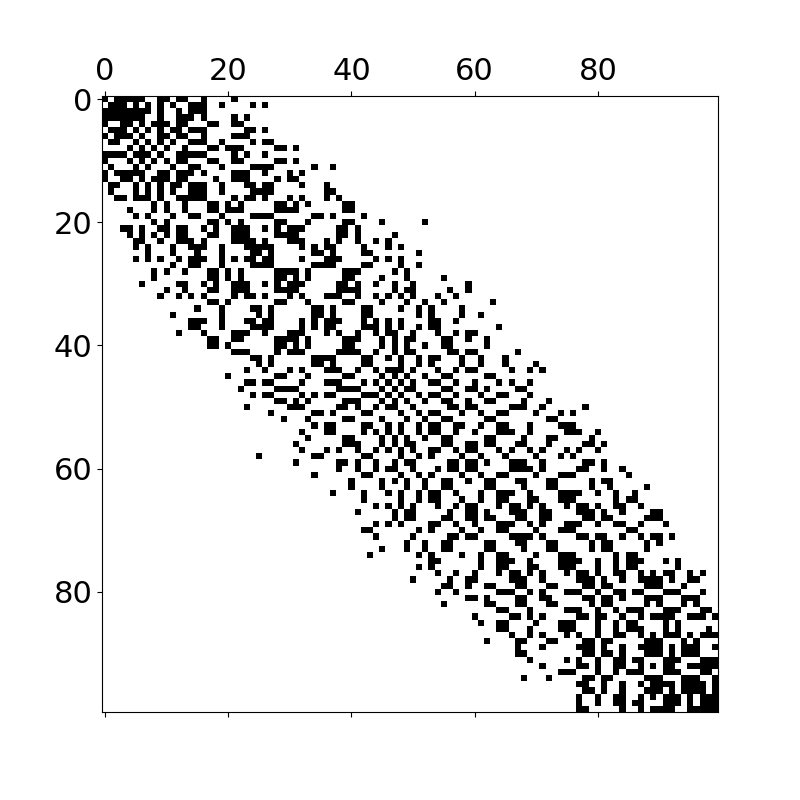
\includegraphics[width=\figordersize\textwidth]{spy_vogel_xorder.png} &
			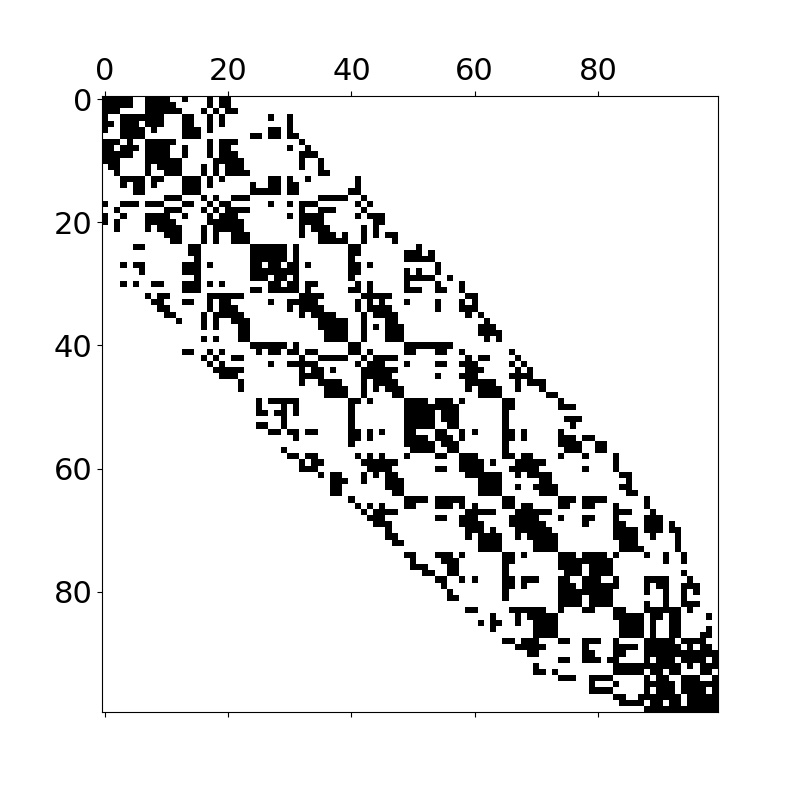
\includegraphics[width=\figordersize\textwidth]{spy_vogel_rcm.png}  \end{tabular} \\
	\end{tabular}
	\caption{Sparsity pattern for weight matrix with 100 interior nodes and a stencil size of 20 nearest neighbors under different point distributions and orderings.}
	\label{orderings}
\end{figure}


%%%%%%%%%%%%%%%%%%%%%%%%%%%%%%%%%%%%%%%%%%%%%%%%%%%%%%%%%%%%%%%%%%%%%%%%%%%%%
\subsection{Forming the Differentiation Matrix}

	Once the points are chosen we pass over each point and construct a stencil of nearest neighbors. Our implementation uses a KD-tree from Scipy's \texttt{spatial} package. After the points are generated and the nearest neighbors calculated they are saved to disk so that they can be later loaded into our CUDA code to form the differentiation matrix. This amounts to constructing and solving $n$ systems of the form
	$$
	\begin{bmatrix}
	A &P\\
	P^T &0
	\end{bmatrix}
	\begin{bmatrix}
	\vec{\omega}\\
	\vec{\lambda}
	\end{bmatrix}
	=
	\begin{bmatrix}
	L\vec{\phi}(\vec{y}) \\
	L\vec{p}(\vec{y}) 
	\end{bmatrix},
	$$
	
	\noindent as described in section \ref{sec_overview_rbffd}. For computational convenience we instead use polynomial basis terms centered at the stencil center. This is convenient because when we evaluate the vector $L\vec{p}(\vec{y})$ almost all of the entries vanish. The only remaining are $Lx^2\vert_{\vec{x}=\vec{0}} = 2$ and $Ly^2\vert_{\vec{x}=\vec{0}} = 2$.
	
	In order to do this efficiently on the GPU we need the host to allocate all the memory the GPU kernels will need in advance for constructing and solving the systems. 
	
	\begin{lstlisting}
cudaMalloc((void**)&full_mat1_root, 
		n*(l_max+pdim)*(l_max+pdim) * sizeof(double));
cudaMalloc((void**)&RHS1_root, 
		n*(l_max+pdim) * sizeof(double));
	\end{lstlisting}
	
	\noindent After the points and nearest neighbors are copied to the device it then uses the thread ID to point to that thread's portion of the array before calling the device functions to construct and solve the system.
	
	\begin{lstlisting}
double* full_mat1 = &full_mat1_root[my_id * (l+pdim)*(l+pdim)];
double* RHS1 = &RHS1_root[my_id * (l+pdim)];
double* weights = &weights_root[my_id * (l+pdim)];
	\end{lstlisting}
	
	We elected to use Gaussian Elimination without pivoting to solve each system. The systems will be small enough that this can be done relatively quickly, and we avoided pivoting to reduce warp divergence. 
	
	Once the weights are calculated they are copied back to the host to be written to disk along with the nearest neighbors matrix which serves to index the weights.
	
	Our serial implementation in python solves these systems directly as well using Scipy's \texttt{linalg} package. Using the PHS RBFs with polynomial basis terms, there is the potential for ill-conditioning or even singularity if the points happen to be arranged particularly badly. We tested using the pseudo inverse (again SciPy's implementaion) instead of Gaussian Elimination but it seemed to make no difference in practice.

%%%%%%%%%%%%%%%%%%%%%%%%%%%%%%%%%%%%%%%%%%%%%%%%%%%%%%%%%%%%%%%
\subsection{Solving the Sparse System}

	Solving the resulting sparse linear system is the most computationally expensive step in the method. The simplest method is to use Gaussian Elimination which is $\mathcal{O}(N^3)$ in general. While this can be improved by taking advantage of the sparsity, iterative methods will be faster for large matrices.
	
	Exploring the methods in chapter 7 of \cite{Ascher2011} the first two iterative methods to consider are the fixed point Jacobi and Gauss-Seidel methods. We have experimentally verified that our differentiation matrices can have eigenvalues very large in magnitude. This violates the convergence criterion for the fixed point methods that the spectral radius is less than one. Indeed testing shows that the Jacobi method diverged. 
	
	The ideal choice would be to use conjugate gradient. It is simple to implement and has very fast convergence. Unfortunately our matrices are not symmetric positive definite (SPD) so conjugate gradient fails. One can artificially force the system $D\vec{u}=\vec{b}$ to be SPD by multiplying by the transpose to get $D^TD\vec{u} = D^T \vec{b}$. Here the matrix $D^TD$ is symmetric positive definite and thus conjugate gradient can be used to solve for $\vec{u}$. The drawback here is that the condition number is greatly increased since $\kappa(D^TD) = \kappa(D)^2$. This has the potential to limit accuracy and is further discussed in section \ref{sec_results}. 
	
	The Stabilized Bi-Conjugate Gradient method (BiCGSTAB) is a variation on conjugate gradient that in theory converges for any matrix. The convergence may be irregular though. It is common to use the incomplete LU as a preconditioner to stabilize the method. In testing BiCGSTAB failed to converge for our matrices unless they had a sufficient preconditioner. 
	
	Lastly we discuss the Generalized Minimum Residual method (GMRES). GMRES is guaranteed to converge. This was confirmed for several large test matrices generated from RBF-FD stencils. While GMRES did not need preconditioning to converge it was found that for sufficiently large problems the incomplete LU preconditioner made convergence quicker.
	
	In our final implementation we used Scipy's sparse solver for matrices smaller than $400 \times 400$ and used GMRES with an incomplete LU preconditioner for larger matrices.

%	\begin{tabular}{|c|c|}
%		Gaussian Elimination & Slow for large systems. \\
%		Jacobi & Spectral radius may be too large and thus it fails to converge. \\
%		Gauss-Seidel & Spectral radius may be too large and thus it fails to converge. \\
%		Conjugate Gradient & The matrix is not SPD. Forcing the system to be SPD squares the condition number.  \\
%		BiCGSTAB & Fails without a decent preconditioner such as the ILU. \\
%		GMRES & Very robust. Convergence is quicker with ILU preconditioning. 
%	\end{tabular}

%%%%%%%%%%%%%%%%%%%%%%%%%%%%%%%%%%%%%%%%%%%%%%%%%%%%%%%%%%%%%%%
%%%%%%%%%%%%%%%%%%%%%%%%%%%%%%%%%%%%%%%%%%%%%%%%%%%%%%%%%%%%%%%
%%%%%%%%%%%%%%%%%%%%%%%%%%%%%%%%%%%%%%%%%%%%%%%%%%%%%%%%%%%%%%%
\section{Results} \label{sec_results}

	For classical finite differences on two dimensional problems their error is given by $\mathcal{O}(h^2)$. Since we do not have a mesh nor an obvious step size this is an inconvenient comparison. Since the number of points is given by roughly $N \approx \pi \frac{1}{h^2}$ this error is equivalent to $\mathcal{O}(N^{-1})$. As stated in Bayona et al. \cite{Flyer2017-2} the rate of convergence of RBF-FD with polyharmonic spline (PHS) RBFs is determined by the degree of the polynomial basis terms. 
	
	We tested this on the problem of the homogeneous steady state heat distribution over the unit disk where the prescribed temperature is given by 
	$$f(\theta) = \cos(2\theta) + \frac{1}{3}\sin(3\theta) + \frac{1}{20}\cos(5\theta)$$
	\noindent for which the analytic solution is known. The convergence rates can be seen figure \ref{convergence}. The top left figure shows the maximum error versus the number of interior points for each degree included in the polynomial basis terms. The stencil sizes were chosen to be twice the number of terms in the polynomial basis (minimum 10). When we include up to 3\textsuperscript{rd} degree polynomial terms we achieve $\mathcal{O}(N^{-1})$ convergence on the error. Adding terms of degree 4 we achieve $\mathcal{O}(N^{-1.8})$. Going up to degree 6 the accuracy of the method becomes limited by the condition number of the matrix. 
	
	We also tested our prediction that using conjugate gradient on the system $D^TD \vec{u}=D^T \vec{b}$ would result in worse accuracy since $\kappa(D^TD) = \kappa(D)^2$. The results can be seen in the first row of figure \ref{convergence}. As expected it had little effect on the lower order stencils, but the degree 5 stencil (for which the error is immediately dominated by the condition number) lost accuracy much more quickly. 
	
%	\begin{figure}
%		\centering
%		\begin{tabular}{cc}
%			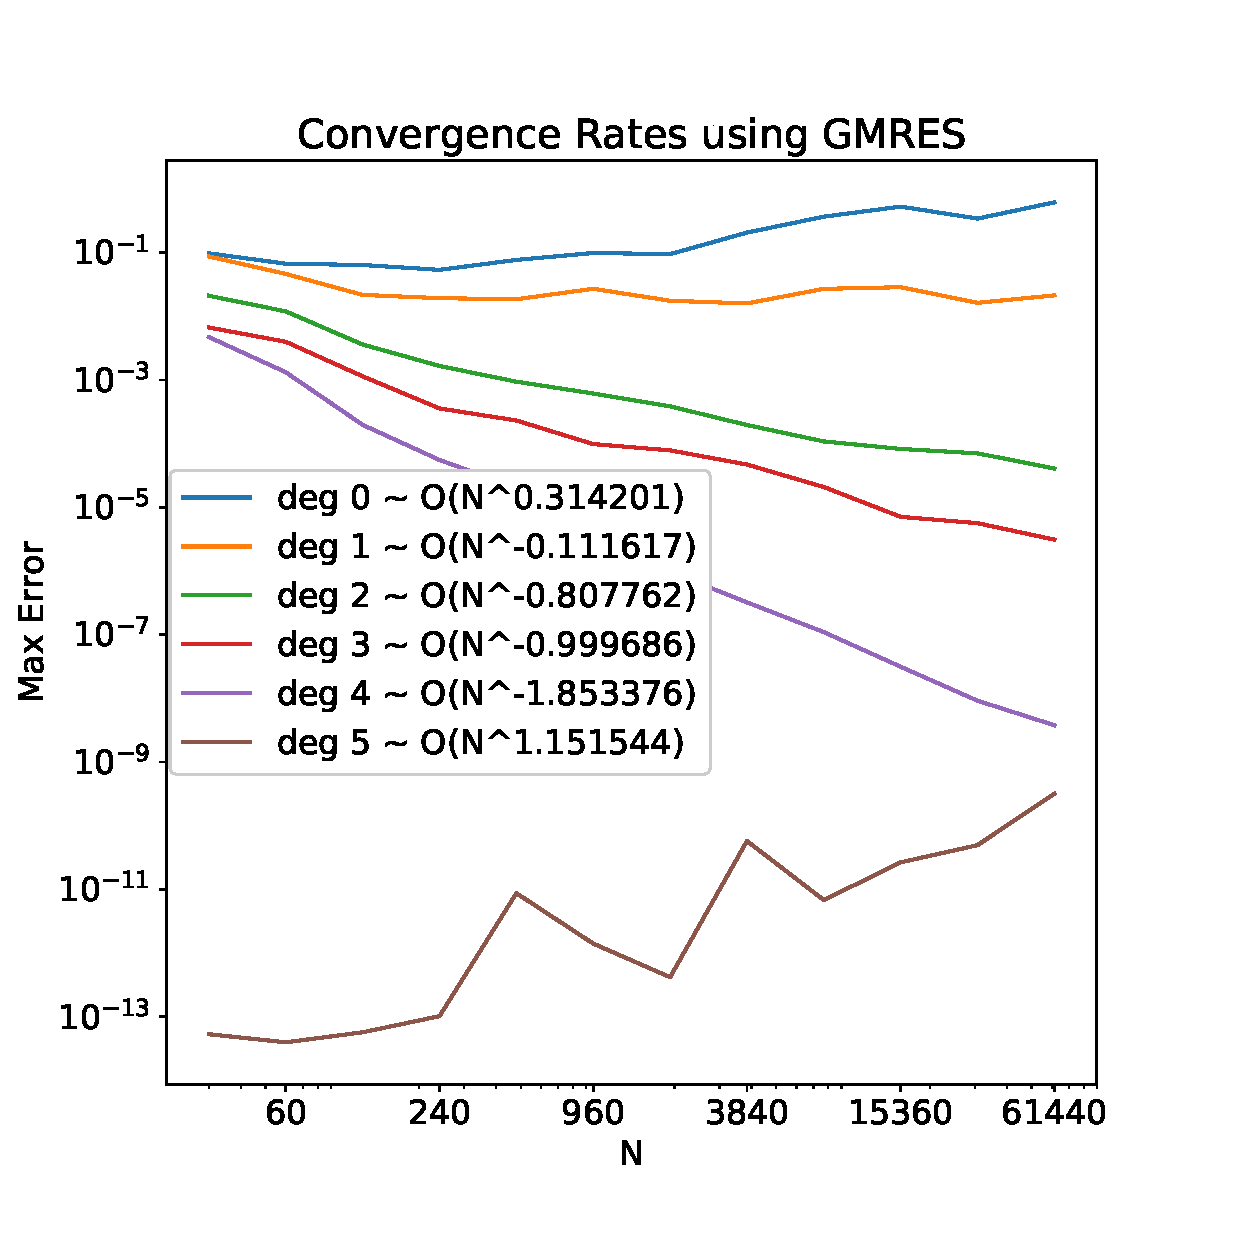
\includegraphics[width=.5\textwidth]{Convergence_GMRES.eps} & 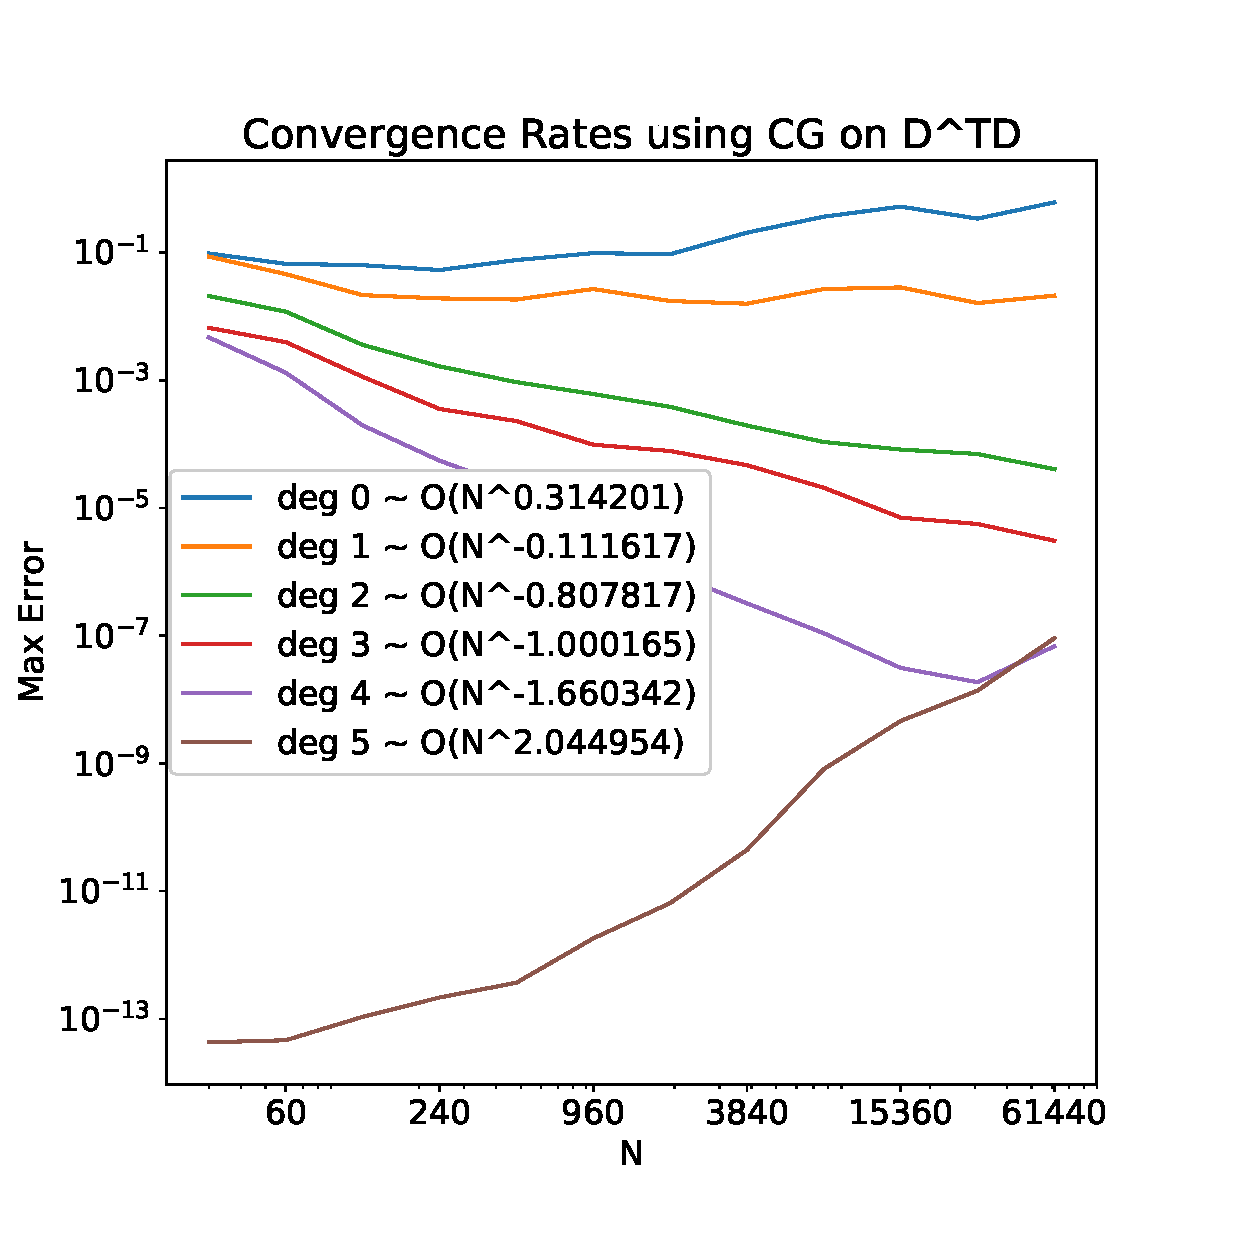
\includegraphics[width=.5\textwidth]{Convergence_Transpose.eps}
%		\end{tabular}
%		\caption{Convergence rates using GMRES on $D\vec{u}=\vec{b}$ vs CG on $D^TD\vec{u}=D^T\vec{b}$ with a stencil size equal to twice the number of polynomial basis terms (minimum of ten).}
%		\label{convergence_cg}
%	\end{figure}
	
	Our testing of different point sets was inconclusive. Convergence of several point sets can be seen in figure \ref{convergence}. Halton points, Vogel nodes and random points have been mentioned previously, but we heretofore have have note mentioned using equally spaced grid points. These are somewhat inflexible in that we cannot choose an arbitrary number of points to fit on a uniform grid inside a circle. Instead we have attempted to choose numbers of points that are relatively close to the numbers we've used for the other point sets. Some point sets were better for smaller numbers of points, but otherwise it seems hard to know in advance which points are best.
	
	\newcommand{\convFigSize}{.45}
	\begin{figure}[hp]
		\centering
		\begin{tabular}{cc}
			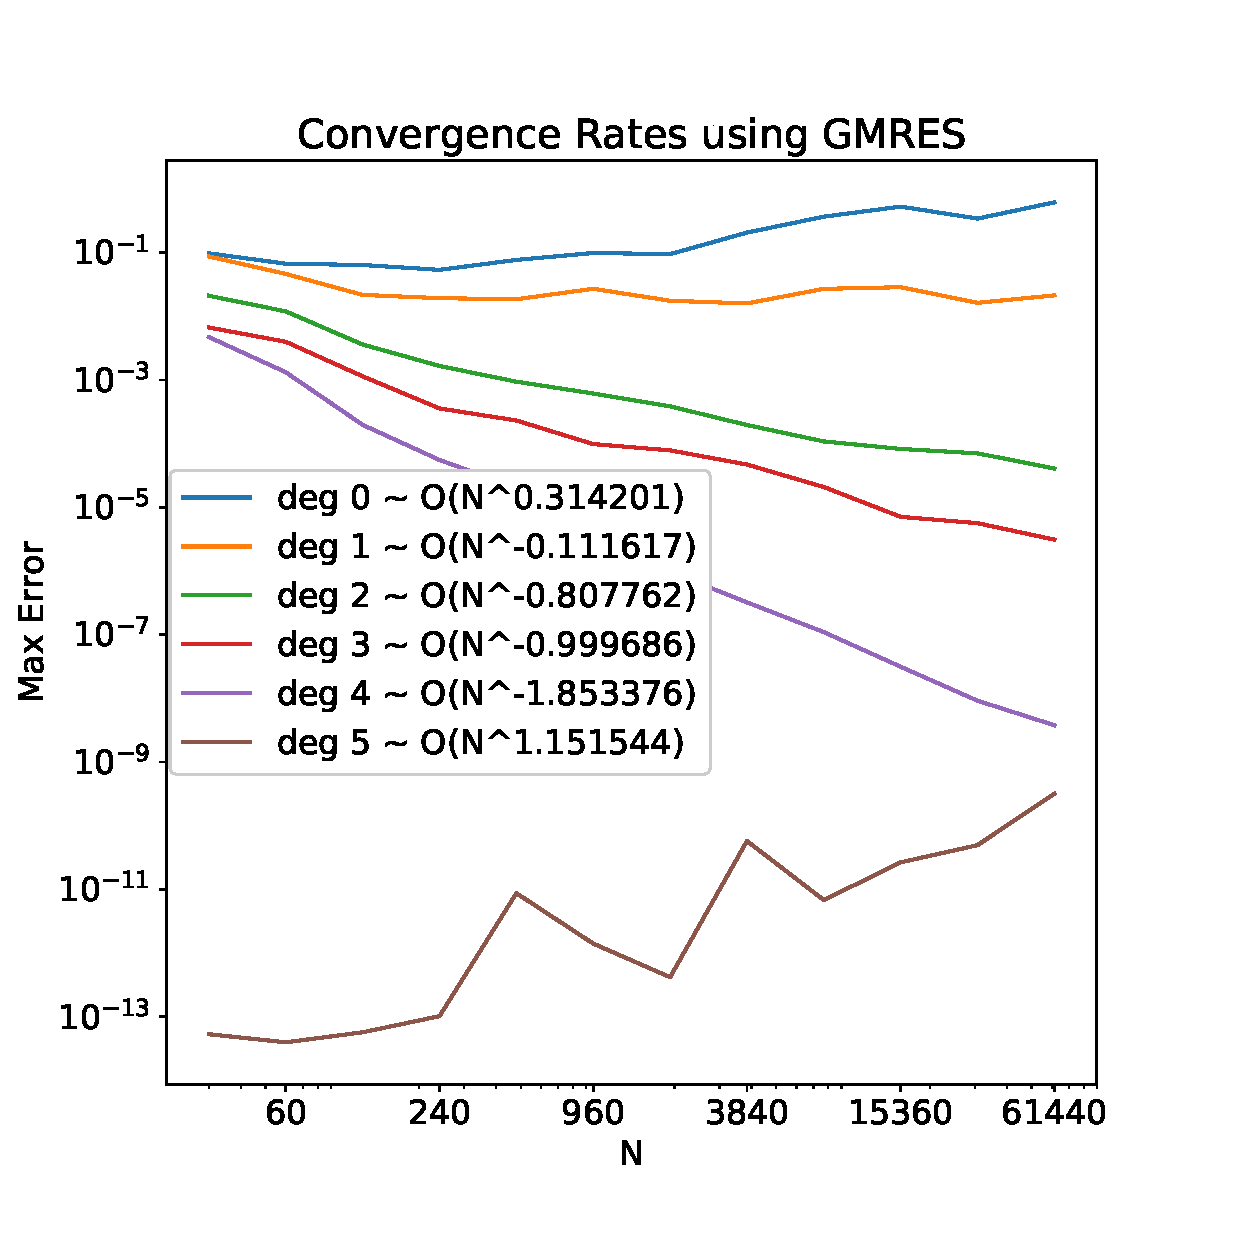
\includegraphics[width=\convFigSize\textwidth]{Convergence_GMRES.eps} & 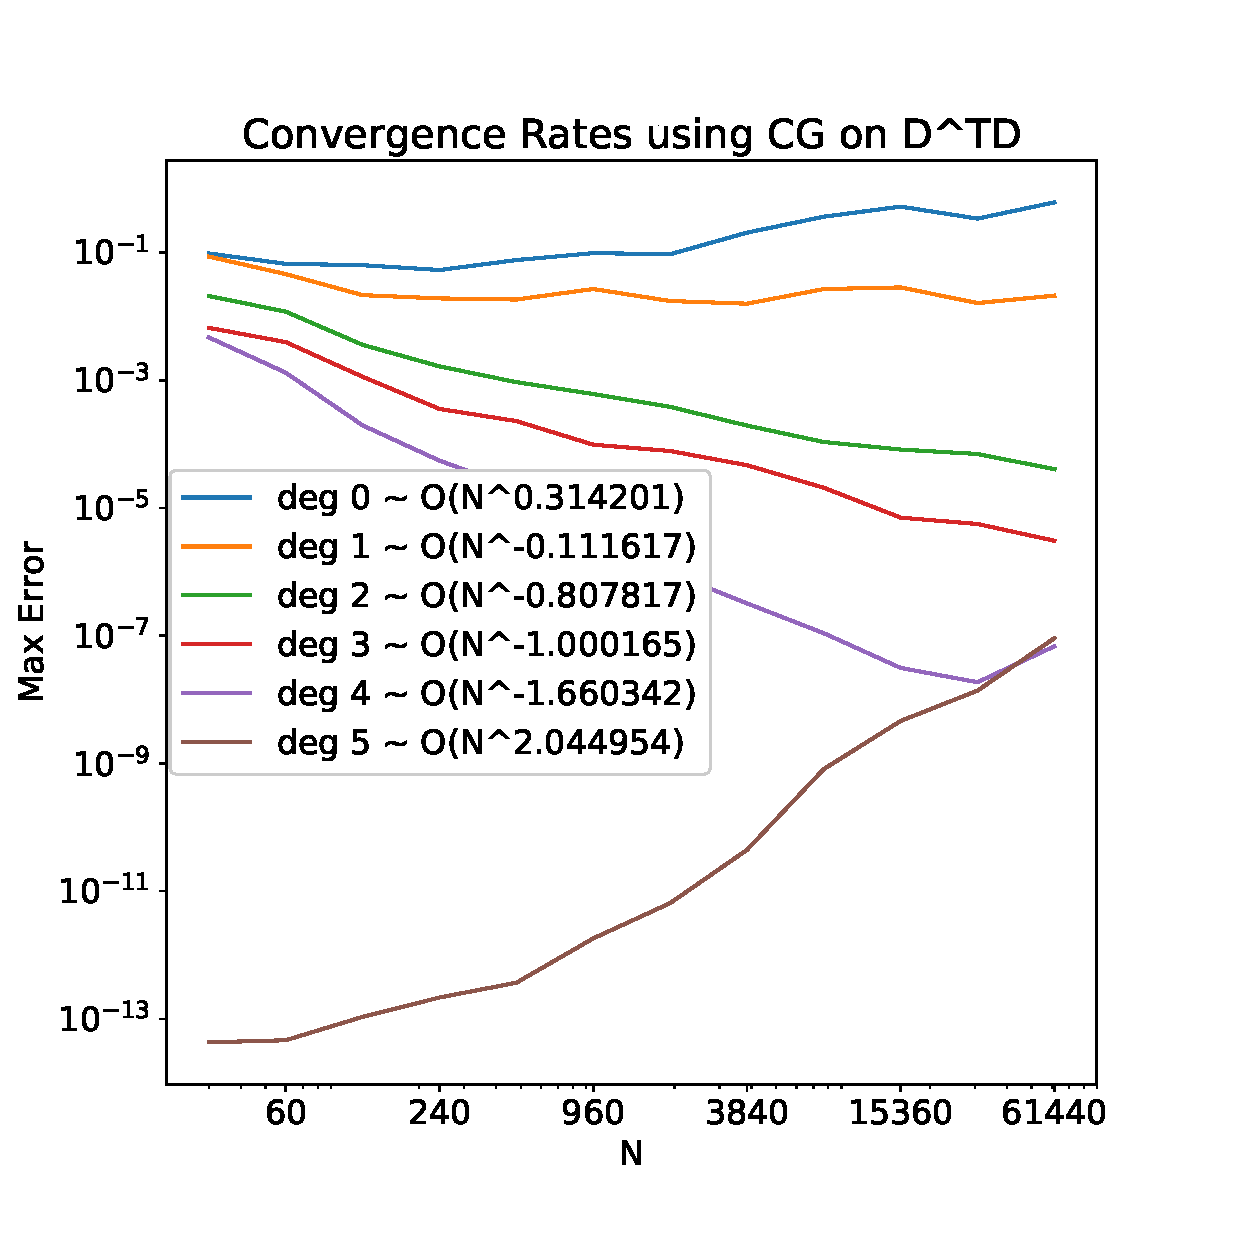
\includegraphics[width=\convFigSize\textwidth]{Convergence_Transpose.eps} \\
			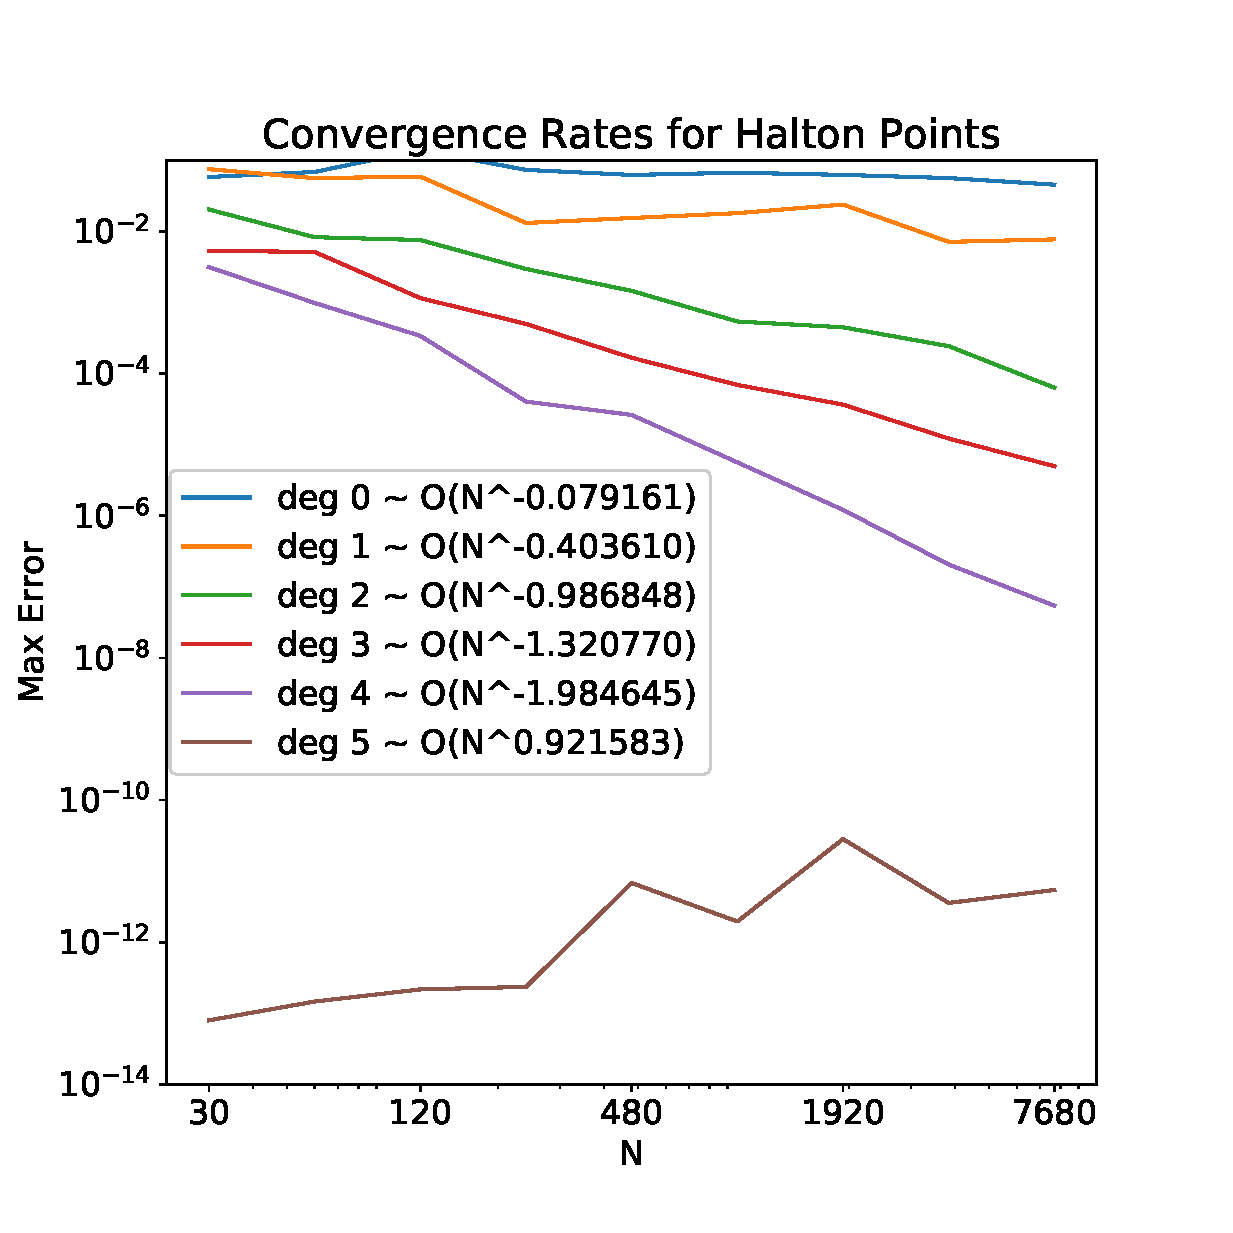
\includegraphics[width=\convFigSize\textwidth]{Convergence_halton.eps} & 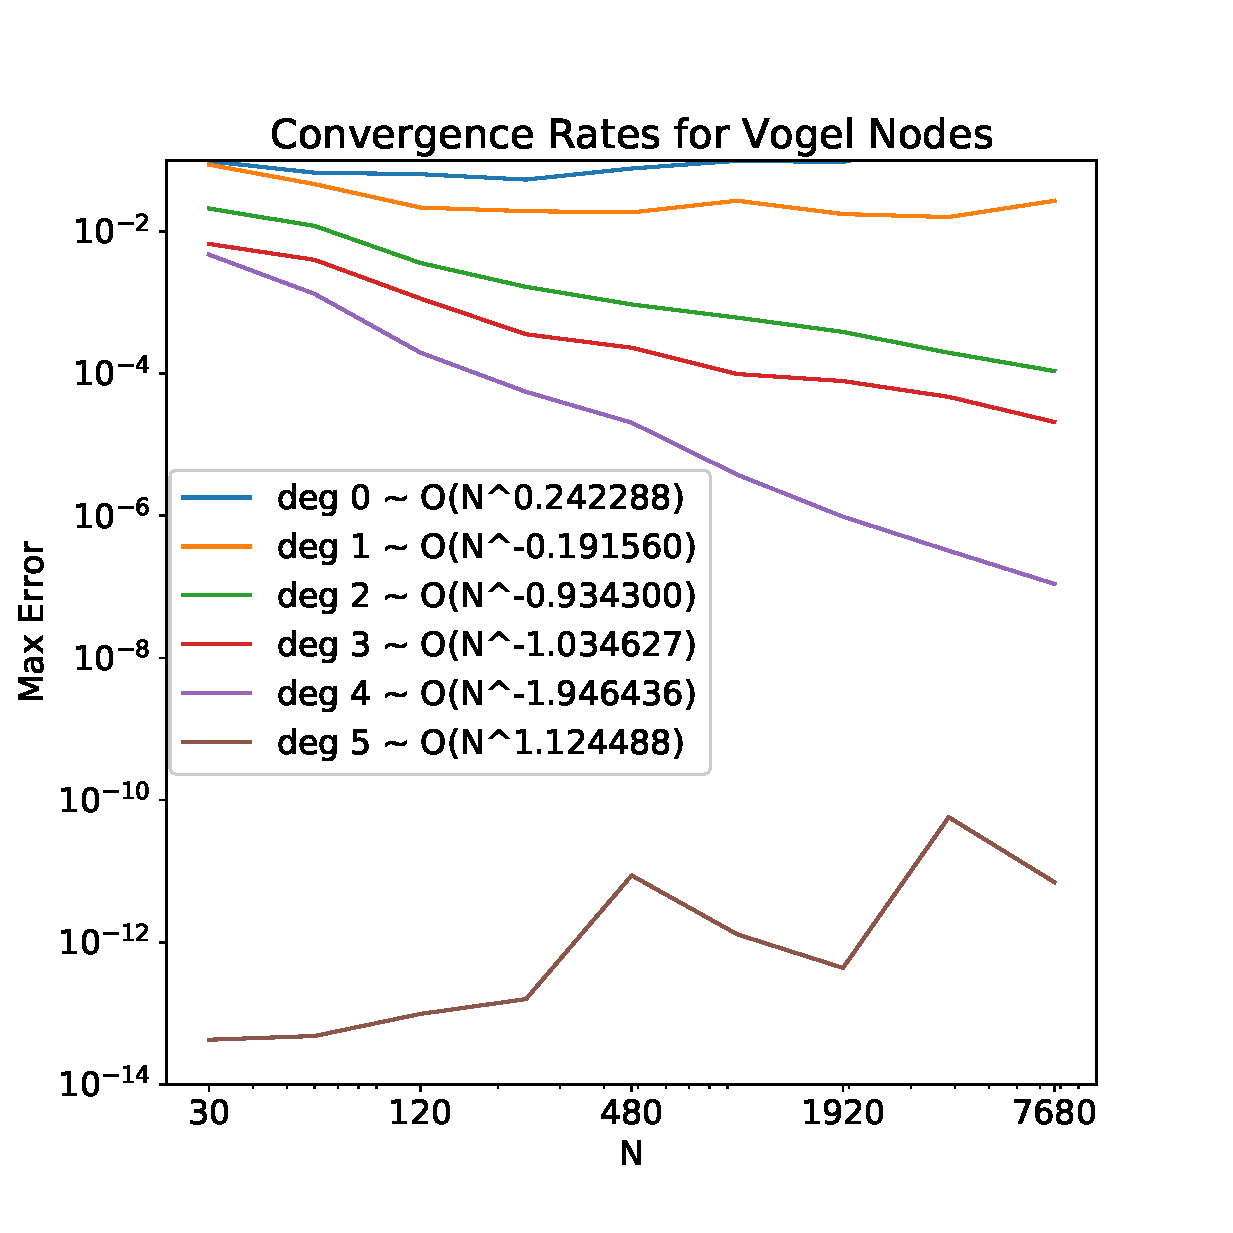
\includegraphics[width=\convFigSize\textwidth]{convergence_vogel.eps} \\
			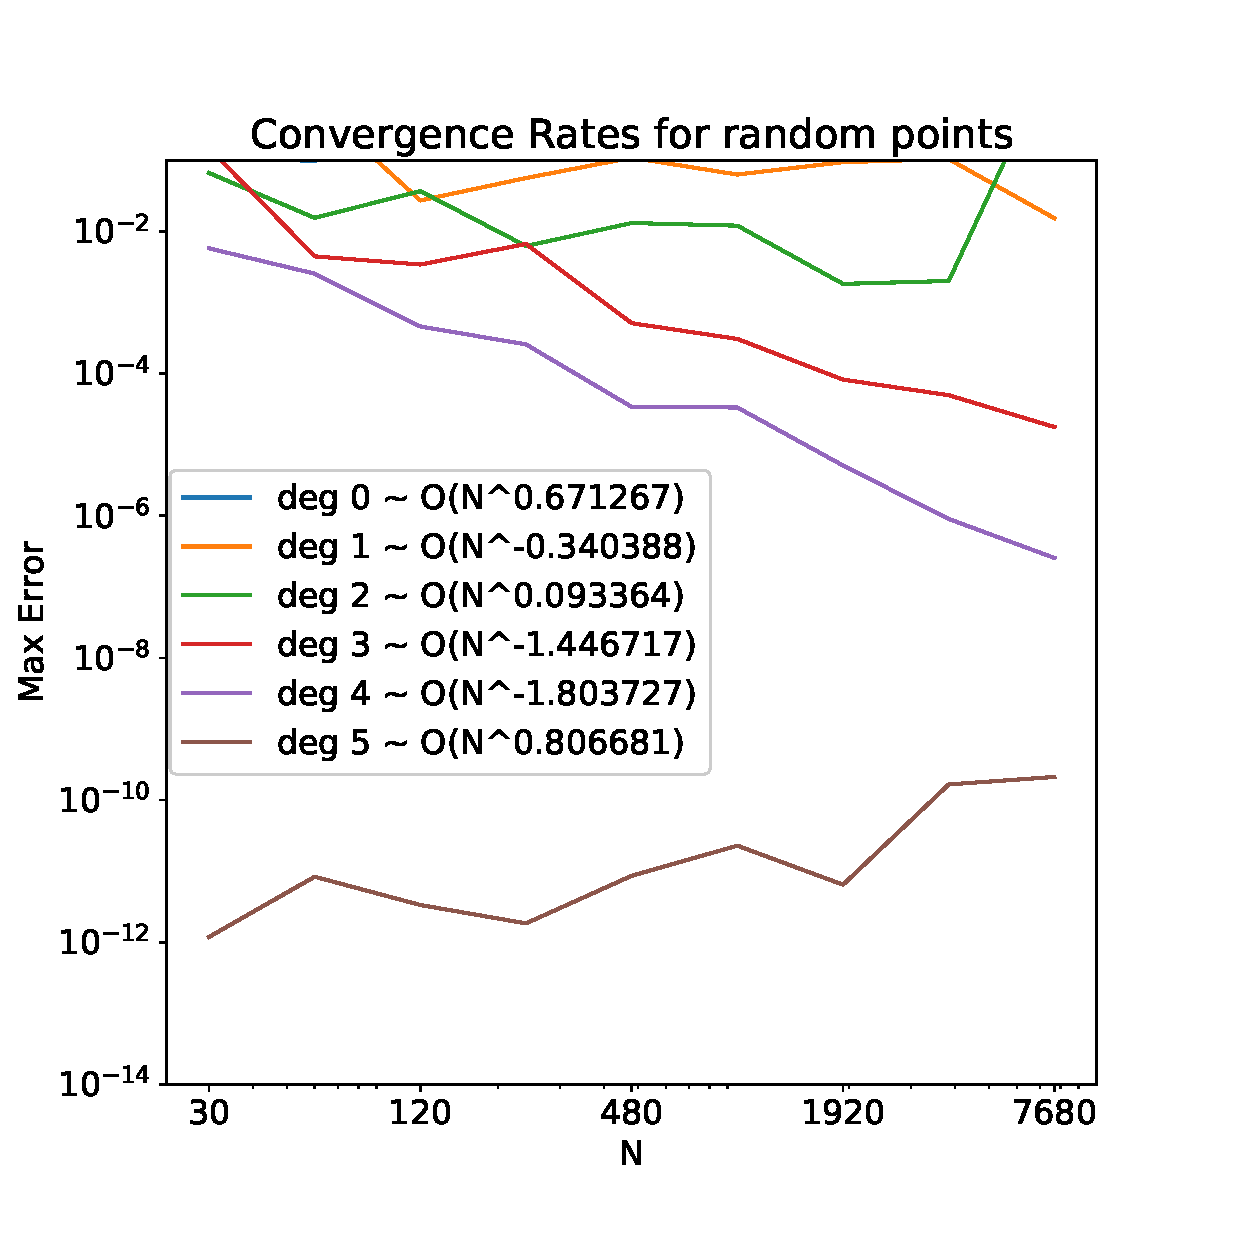
\includegraphics[width=\convFigSize\textwidth]{Convergence_random.eps} & 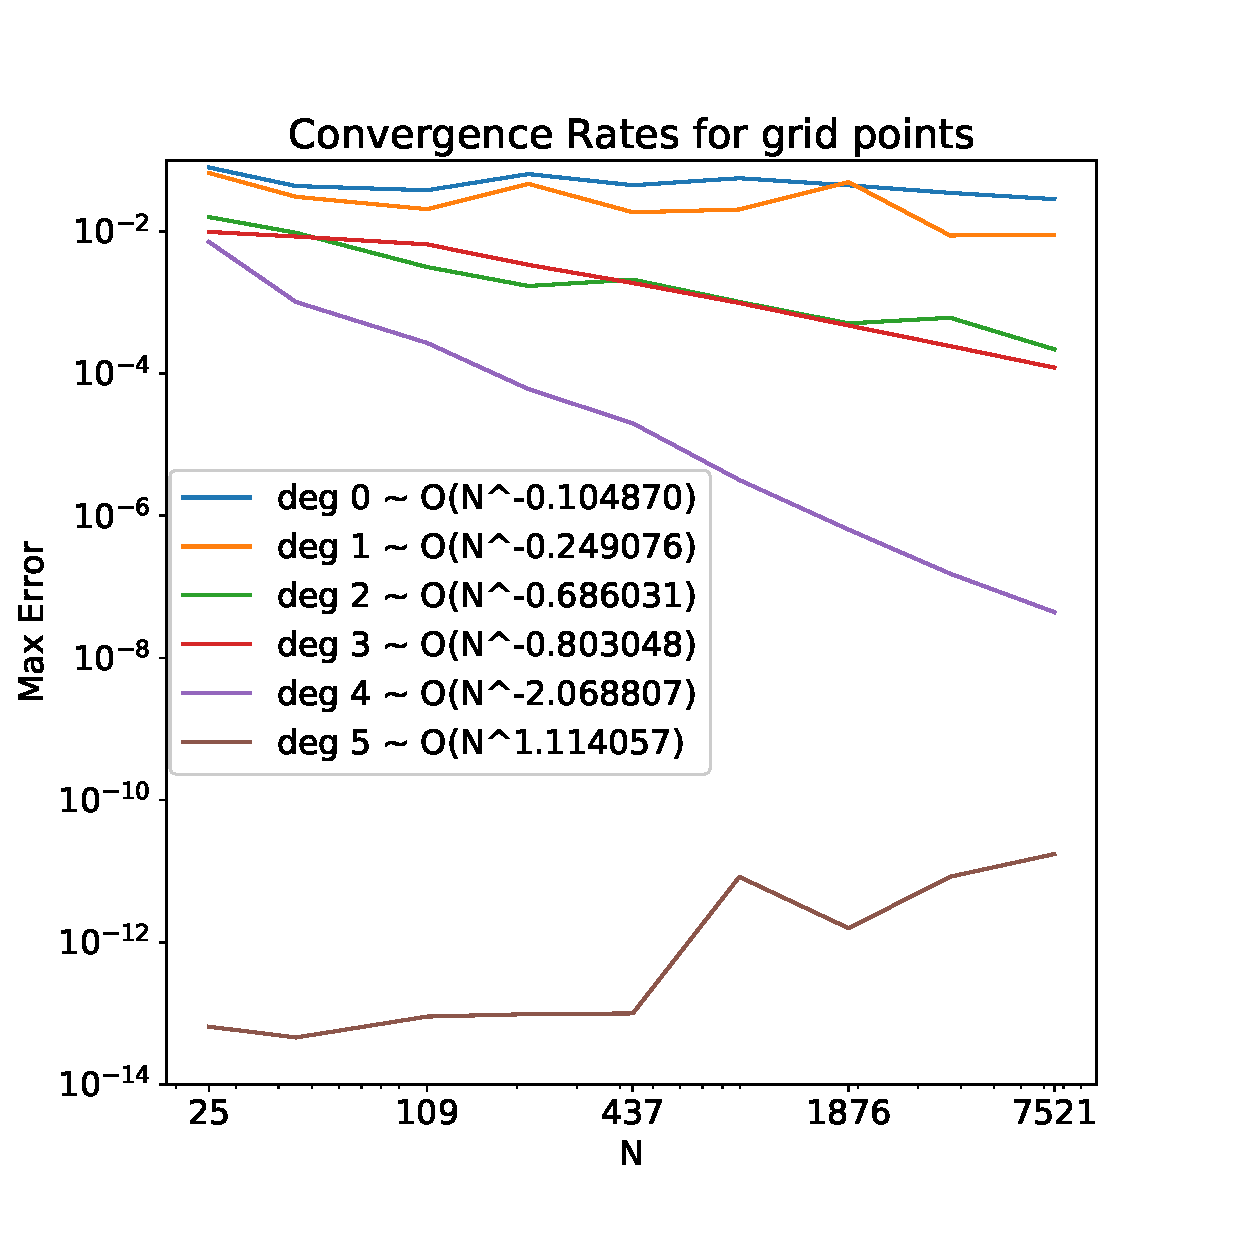
\includegraphics[width=\convFigSize\textwidth]{Convergence_grid.eps} \\
		\end{tabular}
		\caption{Convergence for different point sets.}
		\label{convergence}
	\end{figure}

%%%%%%%%%%%%%%%%%%%%%%%%%%%%%%%%%%%%%%%%%%%%%%%%%%%%%%%%%%%%%%%
%%%%%%%%%%%%%%%%%%%%%%%%%%%%%%%%%%%%%%%%%%%%%%%%%%%%%%%%%%%%%%%
%%%%%%%%%%%%%%%%%%%%%%%%%%%%%%%%%%%%%%%%%%%%%%%%%%%%%%%%%%%%%%%
\section{Conclusions and Future Work}

	While we have greatly reduced the time it takes to generate the differentiation matrix, solving the system is the dominating step and it is still done in serial. Our parallel method would still be useful in explicit time stepping schemes where only matrix vector multiplication is needed. In general it seems RBF-FD is best for high-accuracy solutions for relatively small point sets and for domains that are less amenable to meshes. 
	
	In the future we plan to apply this to time dependent surfaces in three dimensions. We will investigate parallelization of effective preconditioners for BiCGSTAB and GMRES. Ideally we will implement these algorithms on GPUs to take full advantage of modern hardware.

 
% \bigbreak
%\pagebreak
 
\printbibliography

\end{document}
